%%%%%%%%%%%%%%%%%%%%%%%%%%%%%%%%%%%%%%%%%%%%%%%%%%%%%%%%%%%%%%%%%%%%%%
% Lớp 12 | Phương trình mặt phẳng, đường thẳng, mặt cầu | Phương trình đường thẳng trong không gian
% Dạng 2H5?2-4: Vị trí tương đối giữa hai đường thẳng
% Số câu: 53  (sinh tự động bởi tach_cau.py; từ nay thầy sửa trực tiếp file này)
%%%%%%%%%%%%%%%%%%%%%%%%%%%%%%%%%%%%%%%%%%%%%%%%%%%%%%%%%%%%%%%%%%%%%%

%%%%%%%%%%%%%%%% TRẮC NGHIỆM 4 PHƯƠNG ÁN %%%%%%%%%%%%%%%%

% nguồn: Phan1_Lop_12_Hinh_hoc_Chuong_5
\begin{ex}%[2H5H2-4]%[ma:dfb6cce3]
	Trong không gian $Oxyz$, cho đường thẳng $\Delta_{1} \colon \dfrac{x-8}{2}=\dfrac{y+2}{4}=\dfrac{z-3}{m-1}$ và $\Delta_{2} \colon \heva{&x=4+4t\\&y=3-t\\&z=2+2t}$. Giá trị của $m$ để $\Delta_{1}$  và $\Delta_{2}$ vuông góc là
	\choice{$m=1$} 
		{\True $m=-1$} 
		{$m=3$} 
		 {$m=-3$}
	\loigiai{Đường thẳng $\Delta_{1}$  có vectơ chỉ phương $\overrightarrow{u}_{1}=(2; 4; m-1)$.\\
		Đường thẳng  $\Delta_{2}$ có vectơ chỉ phương $\overrightarrow{u}_{2}=(4;-1; 2)$.\\
	Ta có $\Delta_{1}$  và $\Delta_{2}$ vuông góc kh $\overrightarrow{u}_{1} \cdot \overrightarrow{u}_{2}=0 \Leftrightarrow 8-4+2 m-2=0 \Leftrightarrow m=-1$.}
\end{ex}

% nguồn: Phan1_Lop_12_Hinh_hoc_Chuong_5
\begin{ex}%[2H5H2-4]%[ma:281809c1]
	Trong không gian $Oxyz$, cho hai đường thẳng $d \colon \heva{&x=1+t\\&y=2+t\\&z=3-t}$ và $d' \colon \heva{&x=1+2t'\\&y=-1+2t'\\&z=2-2t'}$. Mệnh đề nào sau đây đúng? 
	\choice{Hai đường thẳng $d$ và $d'$ chéo  nhau}
		 {\True Hai đường thẳng $d$ và $d'$ song song với nhau}
		{Hai đường  thẳng $d$ và $d'$ cắt nhau}
		{Hai đường thẳng $d$ và $d'$ trùng nhau} 
	 \loigiai{
		 Đường thẳng $d$ có vectơ chỉ phương $\overrightarrow{u_{1}}=(1; 1;-1)$.\\
		Đường thẳng $d'$ có vectơ chỉ phương $\overrightarrow{u_{2}}=(2;  2;-2)$.\\
		 Ta có $\overrightarrow{u_{2}}=2 \cdot \overrightarrow{u_{1}}$ nên đường thẳng $d$ và $d'$ song song hoặc trùng nhau.\\
		Chọn điểm $M(1; 2; 3)$ thuộc đường thẳng $d$, thay tọa độ điểm $M$ vào phương trình đường thẳng $d'$, ta có $d' \colon \heva{&x=1+2t'\\&y=-1+2t'\\&z=2-2t'}$ vô nghiệm,  vậy $M$ không thuộc đường thẳng $d'$ nên 2 đường thẳng song song nhau.
	 }
\end{ex}

% nguồn: Phan1_Lop_12_Hinh_hoc_Chuong_5
\begin{ex}%[2H5H2-4]%[ma:f9af5b47]
	Trong không gian với hệ trục $Oxyz$, cho đường thẳng $d\colon \dfrac{x - 1}{1} = \dfrac{y}{-1} = \dfrac{z + 2}{1}$ và mặt phẳng $(P)\colon x + 2y + z - 1 = 0$. Biết có hai đường thẳng $d_1$, $d_2$ cùng nằm trên mặt phẳng $(P)$, song song với $d$ và cách $d$ một khoảng  bằng $\sqrt{2}$.\\
	Một đường tròn $(C)$ nằm trên mặt phẳng $(P)$ và  tiếp xúc với cả hai đường thẳng $d_1$, $d_2$. Bán kính của đường tròn $(C)$ bằng
	\choice 
		{\True  $\dfrac{\sqrt{3}}{3}$}
		 {$\dfrac{2\sqrt{2}}{3}$}
		 {$\dfrac{\sqrt{2}}{3}$}
		 {$\dfrac{2\sqrt{3}}{3}$}
	\loigiai{ 
		Đường thẳng $d$ có tâm $I(1;0;-2)$ (lấy $1$  điểm trên $d$).\\
		Gọi $R$ là bán kính đường tròn $(C)$. Vì khoảng cách giữa hai đường thẳng $d_1$, $d_2$ là $2R$, và mỗi đường cách $d$ một khoảng $R$, nên ta có 
		\[ 
		R = \sqrt{2 - d^2(I;  (P))}.
		\] 
		Khoảng cách từ $I(1;0;-2)$ đến mặt phẳng $(P)\colon x + 2y + z  - 1 = 0$ là \[
		\mathrm{d} = \dfrac{|1 + 2 \cdot 0 + (-2) - 1|}{\sqrt{1^2 + 2^2 + 1^2}} =  \dfrac{|-2|}{\sqrt{6}} = \dfrac{2}{\sqrt{6}} = \dfrac{\sqrt{6}}{3}
		 \Rightarrow \mathrm{d}^2 = \left(\dfrac{\sqrt{6}}{3}\right)^2 = \dfrac{6}{9} = \dfrac{2}{3}.
		 \]
		Vậy 
		 \[
		R = \sqrt{2 - \dfrac{2}{3}}  = \sqrt{\dfrac{1}{3}} = \dfrac{\sqrt{3}}{3}.
		 \]
		Do $(C)$ tiếp  xúc với $d_1$, $d_2$ nên $R = \dfrac{\sqrt{3}}{3}$.
	} 
\end{ex}

% nguồn: Phan1_Lop_12_Hinh_hoc_Chuong_5
\begin{ex}%[2H5H2-4]%[ma:6fa34a22]
	Tại một nút giao thông đường bộ có hai con đường. Trên thiết kế, trong không gian $Oxyz$, hai con đường đó tương ứng thuộc hai đường thẳng $\Delta_1\colon  \dfrac{x - 1}{2} = \dfrac{y}{-1} = \dfrac{z + 1}{3}$, $\Delta_2\colon \dfrac{x - 3}{-1} = \dfrac{y + 1}{1} = \dfrac{z}{1}$.
	Khẳng  định nào sau đây là đúng?
	\choice 
		 {$\Delta_1$ và $\Delta_2$ song song với nhau}
		{$\Delta_1$ và $\Delta_2$  trùng nhau}
		{\True $\Delta_1$  và $\Delta_2$ vuông góc với nhau}
		{$\Delta_1$ và $\Delta_2$ không vuông góc với  nhau}
	\loigiai{ 
		$\Delta_1\colon \dfrac{x-1}{2} = \dfrac{y+2}{-1} = \dfrac{z-1}{3}$ có một vectơ chỉ phương là  $\overrightarrow{u}_1=(2;-1;3)$ \\
		$\Delta_2\colon  \dfrac{x-3}{-1} = \dfrac{y-1}{1} = \dfrac{z+2}{1}$ có một vectơ chỉ phương là $\overrightarrow{u}_2=(-1;1;1)$ \\
		Ta  có
		$\overrightarrow{u}_1\perp \overrightarrow{u}_2$ vì $\overrightarrow{u}_1 \cdot \overrightarrow{u}_2 = 2\cdot(-1)  + (-1)\cdot1 + 3\cdot1 = -2 - 1 + 3 = 0$.\\
		Vậy $\Delta_1$ và $\Delta_2$ vuông góc  với nhau.
	 }
\end{ex}

% nguồn: Phan1_Lop_12_Hinh_hoc_Chuong_5
\begin{ex}%[2H5H2-4]%[ma:d2d52ae9]
	Cho hình lập phương $ABCD.A_1B_1C_1D_1$ cạnh bằng $a$. Khoảng  cách giữa $A_1B$ và $B_1C$ bằng
	 \choice
		{\True $\dfrac{a}{\sqrt{3}}$} 
		 {$\dfrac{a}{\sqrt{6}}$}
		{$a\sqrt{3}$} 
		 {$a\sqrt{6}$}
	\loigiai{ 
		Chọn hệ trục tọa độ sao  cho $
		B_1(0;0;0)$, $ A_1(a;0;0)$, $ C_1(0;a;0)$, $ B(0;0;a)$, $  C(0;a;a)$.\\
		Ta  có $
		\vec{A_1B} = (-a;0;a)$, $ \vec{B_1B} = (0;0;a)$,  $ \vec{B_1C} = (0;a;a)$.
		 $$
		\left[\vec{A_1B}, \vec{B_1C}\right] 
		= (-a^2;-a^2;-a^2)=a^2 (-1;-1;-1). 
		$$ 
		 $$
		\left[\vec{A_1B}, \vec{B_1C}\right] \cdot \vec{B_1B}  = a^2(-1;-1;-1) \cdot (0;0;a) = -a^3.
		 $$
		$$ 
		\Rightarrow \mathrm{d}\left(A_1B, B_1C\right) =  \dfrac{a^3}{\sqrt{(-a)^2 + (-a)^2 + (-a)^2}\cdot \sqrt{a^2}} = \dfrac{a}{\sqrt{3}}.
		$$ 
	} 
\end{ex}

% nguồn: Phan1_Lop_12_Hinh_hoc_Chuong_5
\begin{ex}%[2H5H2-4]%[ma:964e0e46]
	Trong không gian với hệ toạ độ $Oxyz$, cho điểm $A(1;2;3)$ và đường thẳng $d  \colon \dfrac{x+1}{2}=\dfrac{y}{1}=\dfrac{z-3}{-2}$. Phương trình đường thẳng $\Delta$ đi qua $A$, vuông góc với đường thẳng $d$ và cắt trục $Oz$ là
	\choice 
		{$\dfrac{x-1}{1}=\dfrac{y-2}{-2}=\dfrac{z-3}{2}$} 
		{\True  $\dfrac{x-1}{1}=\dfrac{y-2}{2}=\dfrac{z-3}{2}$}
		{$\dfrac{x-1}{1}=\dfrac{y-2}{2}=\dfrac{z-3}{4}$} 
		{$\dfrac{x-1}{-1}=\dfrac{y-2}{2}=\dfrac{z-3}{2}$} 
	 \loigiai{
		Đường thẳng $\Delta$ cắt trục $Oz$ tại $B(0;0;b)$  \\
		$\Rightarrow \overrightarrow{BA}=(1;2;3-b)$ là  vectơ chỉ phương của đường thẳng $\Delta$. \\
		Vì $\Delta \perp d$ nên  $\overrightarrow{BA} \cdot \overrightarrow{u}_d=0 \Leftrightarrow 2+2-2(3-b)=0 \Leftrightarrow b=1$. \\
		$\Rightarrow \overrightarrow{BA}=(1;2;2)$.  \\
		Vậy phương  trình $\Delta$ là $\dfrac{x-1}{1}=\dfrac{y-2}{2}=\dfrac{z-3}{2}$.
	} 
\end{ex}

% nguồn: Phan1_Lop_12_Hinh_hoc_Chuong_5
\begin{ex}%[2H5H2-4]%[ma:10926c0e]
	Trong không gian $Oxyz$, cho hai đường thẳng $d_1 \colon  \dfrac{x}{-3} = \dfrac{y+1}{1} = \dfrac{z-3}{1}$ và
	$d_2 \colon \heva{&x = 1 + 3t \\ &y = -2 - t \\ &z = 3 - t}$. 
	Khẳng định nào sau đây đúng? 
	 \choice
		{\True $d_1  \parallel d_2$}
		{$d_1$  và $d_2$ chéo nhau}
		{$d_1  \equiv d_2$}
		{$d_1$ và $d_2$ cắt nhau} 
	\loigiai{ 
		Đường thẳng $d_1 \colon \dfrac{x}{-3} = \dfrac{y+1}{1}  = \dfrac{z-3}{1}$ có vectơ chỉ phương $\overrightarrow{u}_1 = (-3;1;1)$. \\
		Đường thẳng $d_2 \colon\heva{&x = 1+3t \\ &y  = -2 - t \\& z = 3 - t}$ và có vectơ chỉ phương $\overrightarrow{u}_2 = (3;-1;-1)$. \\
		Ta có $\overrightarrow{u}_1 = -\overrightarrow{u}_2$ và $A \notin d_2$. Do đó $d_1 \parallel d_2$. 
	} 
\end{ex}

% nguồn: Phan1_Lop_12_Hinh_hoc_Chuong_5
\begin{ex}%[2H5H2-4]%[ma:7a4a08aa]
	Trong hệ toạ độ  $Oxyz$, cho hai đường thẳng $\Delta_{1}\colon \dfrac{x-2}{1}=\dfrac{y+3}{-2}=\dfrac{z-5}{3}$ và $\Delta_{2}\colon
	 \heva{&
	x=3-t  \\&
	y=2+2t  \\&
	 z=mt}.$
	Giá  trị của $m$ để hai đường thẳng $\Delta_{1}$ và $\Delta_{2}$ song song?
	 \choice
		{$m=1$} 
		 {$m=-1$}
		{$m=3$} 
		{\True $m=-3$} 
	\loigiai{Đường thẳng $\Delta_{1}$ đi qua điểm $M(2;-3;5)$, có vectơ chỉ phương $\overrightarrow{u}_{1}=(1;-2;3)$; đường thẳng $\Delta_{2}$ đi qua  điểm $N(3;2;0)$, có vectơ chỉ phương $\overrightarrow{u}_{2}=(-1;2;m)$.\\
		 Hai đường thẳng $\Delta_{1}$ và $\Delta_{2}$ song song khi và chỉ khi $\overrightarrow{u}_{1}$ và $\Delta_{2}$ cùng phương, đồng thời điểm $N(3;2;0)$ không thuộc đường thẳng $\Delta_{1}$.\\
		Ta thấy, hai vectơ  $\overrightarrow{u}_{1}$ và $\Delta_{2}$ và $\overrightarrow{u}_{2}$ cùng phương khi và chỉ khi $$\dfrac{-1}{1}=\dfrac{2}{-2}=\dfrac{m}{3}\Leftrightarrow m=-3.$$
	Vì điểm $N(3;2;0)$  không thuộc đường thẳng $\Delta_{1}$ nên $m=-3$ thỏa đề bài. }
\end{ex}

% nguồn: Phan1_Lop_12_Hinh_hoc_Chuong_5
\begin{ex}%[2H5H2-4]%[ma:a8474dba]
	Trong không gian tọa độ $Oxyz$, xét vị  trí tương đối của hai đường thẳng
	$\Delta_{1}  \colon \dfrac{x-1}{2}=\dfrac{y+1}{2}=\dfrac{z}{3}$, $\Delta_{2} \colon \dfrac{x-3}{-1}=\dfrac{y-3}{-2}=\dfrac{z+2}{1}$?
	\choice{$\Delta_{1}$ song song  với $\Delta_{2}$}
		 {$\Delta_{1}$ chéo với $\Delta_{2}$}
		{\True  $\Delta_{1}$ cắt $\Delta_{2}$}
		{$\Delta_{1}$ trùng với $\Delta_{2}$} 
	\loigiai{ 
		Vì $\dfrac{2}{-1} \neq \dfrac{2}{-2}$ nên vectơ chỉ phương $\overrightarrow{u_{1}}=(2; 2; 3)$ của đường thẳng $\Delta_{1}$ không cùng phương với vectơ chỉ phương $\overrightarrow{u_{2}}=(-1;-2; 1)$ của $\Delta_{2}$ suy ra $\Delta_{1}$ chéo với $\Delta_{2}$ hoặc $\Delta_{1}$ cắt  $\Delta_{2}$.\\
		Lấy $M(1;-1; 0) \in \Delta_{1}$, $N(3; 3;-2) \in \Delta_{2}$. Ta có  $\overrightarrow{M N}=(2; 4;-2)$.
		Khi đó $\left[\overrightarrow{u_{1}}, \overrightarrow{u_{2}}\right] \cdot \overrightarrow{M N}=0$.  \\
	Vậy $\Delta_{1}$ cắt  $\Delta_{2}$.}
\end{ex}

% nguồn: Phan1_Lop_12_Hinh_hoc_Chuong_5
\begin{ex}%[2H5H2-4]%[ma:22a4ad96]
	Trong không gian với hệ trục tọa độ  $Oxyz$, cho hai đường thẳng $d_{1} \colon \dfrac{x-1}{2}=\dfrac{y-7}{1}=\dfrac{z-3}{4}$ và $d_{2} \colon \dfrac{x}{3}=\dfrac{y-3}{-2}=\dfrac{z+4}{1}$ cắt nhau tại điểm $M$ có tọa độ bằng
	\choice{$M(0;3;-4)$} 
		 {$M(1;7;3)$}
		{\True  $M(-3;5;-5)$}
		{$M(3;-5;5)$} 
	 \loigiai{
		Đường thẳng $d_1$ có phương  trình tham số $\heva{&x=1+2t \\ &y=7+t \\ &z=3+4t}$. \\
		Đường thẳng $d_2$  có một phương trình tham số $\heva{&x=3t' \\ &y=3-2t' \\ &z=-4+t'}$. \\
		 Xét hệ phương trình $$\heva{&3t'=1+2t\\&3-2t'=7+t\\&-4+t'=3+4t}\Leftrightarrow\heva{&t'=-1\\&t=-2}.$$
	Suy ra hai đường thẳng cắt nhau  tại điểm $M(-3;5;-5)$.}
\end{ex}

% nguồn: Phan1_Lop_12_Hinh_hoc_Chuong_5
\begin{ex}%[2H5H2-4]%[ma:1f20fbb9]
	Trong không gian với hệ toạ độ $Oxyz$, cho điểm $A(1;2;0)$. Phương trình đường thẳng  $\Delta$ đi qua $A$, vuông góc và cắt trục $Ox$ là
	\choice 
		{$\heva{&x=1 \\ &y=t \\ &z=t}$} 
		{$\heva{&x=1-t \\ &y=2+t \\  &z=0}$}
		{$\heva{&x=1+t \\ &y=2+t \\  &z=0}$}
		{\True $\heva{&x=1  \\ &y=t \\ &z=0}$}
	\loigiai{ 
		Gọi $M(m;0;0)$ là giao điểm của $\Delta$ với trục  $Ox$.\\
		Khi đó  $\overrightarrow{AM}=(m-1;-2;0)$ và $\overrightarrow{i}=(1;0;0)$.\\
		Mà $\overrightarrow{AM}\cdot \overrightarrow{i}=0$ nên  $m-1=0\Leftrightarrow m=1$. Suy ra $M(1;0;0)$ và $\overrightarrow{AM}=(0;-2;0)$.\\
		Đường thẳng $\Delta$ đi qua điểm $M(1;0;0)$ và có vectơ chỉ phương $\overrightarrow{u}=-\dfrac{1}{2}\overrightarrow{AM}=(0;1;0)$ có phương trình tham  số là
		$$\heva{&x=1 \\ &y=t  \\ &z=0.}$$
	 }
\end{ex}

% nguồn: Phan1_Lop_12_Hinh_hoc_Chuong_5
\begin{ex}%[2H5H2-4]%[ma:8afec6cd]
	Trong không gian với hệ tọa độ $Oxyz$, cho hai đường thẳng thẳng $d \colon \dfrac{x}{2}=\dfrac{y-1}{-1}=\dfrac{z+2}{1}$ và  $d' \colon \heva{&x=-1+2t\\&y=1+t\\&z=3}$. Khẳng định nào sau đây là khẳng định đúng?
	\choice{\True $d$ và $d'$ chéo nhau} 
		{$d$ song song với  $d'$}
		{$d$  trùng với $d'$}
		{$d$ cắt  $d'$ tại điểm $A(0; 1;-2)$}
	\loigiai{ 
		Làm bằng  phương pháp tự luận:\\
		Đường thẳng $d$ đi qua điểm $M(0;1;-2)$ và  có vectơ chỉ phương $\vec{u}=(2;-1; 1)$.\\
		Đường thẳng $d'$ đi  qua điểm $N(-1; 1; 3)$ và có vectơ chỉ phương $\vec{v}=(2;1;0)$.
		$\Rightarrow[\vec{u},\vec{v}]=(-1;2;4)$,\\$\overrightarrow{MN}=(-1;0;5) \Rightarrow[\vec{u},\vec{v}] \cdot \overrightarrow{M N}=21 \neq  0 \Rightarrow d$ và $d'$ chéo nhau.\\
		Làm bằng phương  pháp trắc nghiệm:\\
		Ta có: $\vec{u}=(2;-1;1)$ và $\vec{v}=(2;1;0)$ không  cùng phương $\Rightarrow$ Đáp án $\mathrm{B}$, $\mathrm{C}$ loại.\\
	Điểm $A(0;1;-2)$ không thuộc đường  thẳng $d' \Rightarrow$ Đáp án D loại.}
\end{ex}

% nguồn: Phan1_Lop_12_Hinh_hoc_Chuong_5
\begin{ex}%[2H5H2-4]%[ma:1fa7dc3c]
	Cho đường thẳng $d\colon \heva{&  x=-1+2 t \\ & y=-t \\& z=-2-t}$.
	Trong các  đường thẳng sau, đường thẳng nào vuông góc với $d$?
	\choice 
		{\True $d_1\colon\heva{&x=3t'  \\ &y=1+t' \\ & z=5t'}$}
		{$d_2\colon\heva{&x=2  \\ &y=2+t' \\ & z=1+t'}$}
		 {$d_3\colon\dfrac{x-2}{3}=\dfrac{y}{2}=\dfrac{z-1}{-5}$}
		{$d_4\colon \dfrac{x+2}{2}=\dfrac{y}{-1}=\dfrac{z+1}{2}$} 
	\loigiai{ 
		$d$ có vectơ chỉ phương là  $\overrightarrow{u}=(2; -1; -1)$.\\
		$d_1$ có vectơ chỉ phương  là $\overrightarrow{u}_1=(3; 1; 5)$.\\
		Ta có $\overrightarrow{u}\cdot \overrightarrow{u}_1=2\cdot3-1\cdot1-1\cdot5=0$  nên $d\perp d_1$.
	 }
\end{ex}

% nguồn: Phan1_Lop_12_Hinh_hoc_Chuong_5
\begin{ex}%[2H5H2-4]%[ma:2308364b]
	Trong không gian $Oxyz$, cho  hai đường thẳng $d_1\colon \dfrac{x-1}{2}=\dfrac{y-7}{1}=\dfrac{z-3}{4}$ và\\
	$d_2\colon \dfrac{x}{3}=\dfrac{y-3}{-2}=\dfrac{z+4}{1}$ cắt nhau tại điểm $M$ có tọa độ bằng 
	\choice 
		{$M(0;3;-4)$} 
		 {$M(1;7;3)$}
		{\True $M(-3;5;-5)$} 
		{$M(3;-5;5)$} 
	 \loigiai{
		Gọi $M=d_1 \cap d_2$.\\ 
		Phương  trình tham số của $d_1$ là $ d_1\colon \heva{&x=2t+1 \\&y=t+7\\&z=4t+3.}$\\
		Vì $M \in d_1$ nên tọa độ $M$ có dạng $M(2t+1;  t+7; 4t+3)$.\\
		Vì $M \in d_2$ nên thay tọa độ  $M$ vào phương trình $d_2$ ta được
		\begin{eqnarray*}
			&&\dfrac{2t+1}{3}=\dfrac{t+4}{-2}=\dfrac{4t+7}{1} \\ 
			 &\Leftrightarrow& \heva{&-2(2t+1)=3(t+4)\\&2t+1=3(4t+7)}\\
			&\Leftrightarrow&\heva{&-4t-2=3t+12\\&2t+1=12t+21} \\ 
			&\Leftrightarrow&\heva{&-7t=14\\&-10t=20}\\ 
			 &\Leftrightarrow& t=-2.
		\end{eqnarray*}
		Vậy  giao điểm $M$ có tọa độ là $(-3;5;-5)$.
	} 
\end{ex}

% nguồn: Phan1_Lop_12_Hinh_hoc_Chuong_5
\begin{ex}%[2H5H2-4]%[ma:ea6f81f9]
	Trong không gian với hệ toạ độ $Oxyz$, cho điểm $A(-1;1;0)$. Phương trình đường thẳng $\Delta$ đi qua $A$, cắt  trục $Ox$, sao cho góc tạo bởi $\Delta$ với hai trục $Ox$, $Oy$ bằng nhau là
	 \choice
		{$\heva{&x=-1+2t \\  &y=1-t \\ &z=0}$}
		{$\heva{&x=-1+t \\ &y=1-2t \\ &z=0}$} 
		{\True $\heva{&x=-1+t \\ &y=1-t \\  &z=0}$}
		{$\heva{&x=t \\ &y=1-t \\ &z=0}$} 
	\loigiai{ 
		Gọi $M(m;0;0)$ là giao điểm  của $\Delta$ với trục $Ox$.\\
		Khi đó $\overrightarrow{AM}=(m-1;-2;0)$ và $\overrightarrow{i}=(1;0;0)$, $\overrightarrow{j}=(0;1;0)$.\\ 
		Theo  đề
		\begin{eqnarray*}
			&&\cos\left(\Delta,Ox\right)=\cos\left(\Delta,Oy\right)\\ 
			&\Leftrightarrow&\left| \cos\left(\overrightarrow{AM},\overrightarrow{i}\right)\right|  =\left|\cos\left(\overrightarrow{AM},\overrightarrow{j}\right)\right|\\
			 &\Leftrightarrow&\dfrac{\left|\overrightarrow{AM}\cdot\overrightarrow{i}\right|}{\left|\overrightarrow{AM}\right|\cdot \left|\overrightarrow{i}\right|}=\dfrac{\left|\overrightarrow{AM}\cdot\overrightarrow{j}\right|}{\left|\overrightarrow{AM}\right|\cdot \left|\overrightarrow{j}\right|}\\
			&\Leftrightarrow&\dfrac{\left|m+1\right|}{\sqrt{m^2+2m+2}}=\dfrac{\left|-1\right|}{\sqrt{m^2+2m+2}}\\ 
			 &\Leftrightarrow&\left|m+1\right|=1\\
			&\Leftrightarrow&\hoac{&m=0\\&m=-2.} 
		\end{eqnarray*}
		Với $m=0$ suy ra $\Delta$ đi qua điểm $A(-1;1;0)$  và có vectơ chỉ phương $\overrightarrow{AM}=(1;-1;0)$ có phương trình tham số là
		 $$\heva{&x=-1+t \\ &y=1-t \\ &z=0.}$$
		Với $m=-2$ suy ra $\Delta$ đi qua điểm $A(-1;1;0)$ và có vectơ chỉ phương $\overrightarrow{AM}=(-1;-1;0)$ có phương trình  tham số là
		$$\heva{&x=-1-t \\  &y=1-t \\ &z=0.}$$
	 }
\end{ex}

% nguồn: Phan1_Lop_12_Hinh_hoc_Chuong_5
\begin{ex}%[2H5H2-4]%[ma:74debd10]
	Cho hình chóp $S.ABCD$ có đáy $ABCD$ là tam giác vuông với $AB = AC = 2$. Cạnh bên $SA$ vuông góc với đáy và $SA = 3$. Gọi  $M$ là trung điểm của $SC$. Tính khoảng cách giữa $AM$ và $BC$.
	 \choice
		{$\dfrac{\sqrt{3}}{2}$} 
		 {$\dfrac{2\sqrt{3}}{3}$}
		{\True  $\dfrac{3\sqrt{22}}{11}$}
		 {$\dfrac{\sqrt{22}}{6}$}
	\loigiai{ 
		Đặt hệ trục tọa độ sao  cho $
		A(0;0;0)$, $ B(2;0;0)$,  $ C(0;2;0)$, $ S(0;0;3)$.\\
		Điểm $M \left(0;1;\dfrac{3}{2}\right)$,  ta có
		$ 
		 \vec{AM} = \left(0;1;\dfrac{3}{2}\right)$, $ \vec{BC} = (-2;2;0)$. \\
		Gọi 
		$ \vec{n} = \left[\vec{AM}, \vec{BC}\right] = (-3;  -3; 2)$.\\
		Mặt phẳng $(P)$ qua điểm $B(2;0;0)$ và nhận $\vec{n}$ làm véc-tơ pháp tuyến có  phương trình
		$$ 
		-3(x - 2) - 3y + 2z = 0 \Rightarrow -3x  - 3y + 2z + 6 = 0.
		 $$
		 Ta có
		 $$
		\mathrm{d}(AM, BC) = \mathrm{d}(A, (P)) = \dfrac{|-3\cdot 0 -3\cdot 0 + 2\cdot 0 + 6|}{\sqrt{(-3)^2 + (-3)^2 + 2^2}} = \dfrac{6}{\sqrt{22}} =  \dfrac{3\sqrt{22}}{11}.
		 $$
	} 
\end{ex}

% nguồn: Phan1_Lop_12_Hinh_hoc_Chuong_5
\begin{ex}%[2H5H2-4]%[ma:9e949a57]
	Trong  không gian với hệ toạ độ $Oxyz$, cho điểm $A(1;0;3)$. Viết phương trình đường thẳng $\Delta$ đi qua $A$, cắt hai trục $Ox$, $Oz$ tại $M$, $N$ sao cho $\overrightarrow{AM}=2\overrightarrow{AN}$.
	\choice 
		 {$\heva{&x=-1-2t \\ &y=0 \\ &z=3t}$}
		{\True $\heva{&x=-1+2t  \\ &y=0 \\ &z=3t}$}
		{$\heva{&x=1+t  \\ &y=0 \\ &z=3+3t}$}
		{$\heva{&x=1+2t \\ &y=0 \\  &z=3t}$}
	\loigiai{ 
		 Gọi: $M(m;0;0)$ và $N(0;0;n)$ $(m \ne n)$. \\
		Ta có $\overrightarrow{AM}=(m-1;0;-3),\  \overrightarrow{AN}=(-1;0;n-3)$. \\
		Theo đề  bài: $\overrightarrow{AM}=2\overrightarrow{AN} \Leftrightarrow
		\heva{m-1 &= -2  \\ -3 &= 2n-6} \Leftrightarrow
		\heva{&m=-1 \\ &n=\dfrac{3}{2}}.  \\
		\Rightarrow  M(-1;0;0),\ N\left(0;0;\dfrac{3}{2}\right)$. \\
		 Vậy phương trình $\Delta \colon$ $\heva{&x=-1+2t \\ &y=0 \\ &z=3t}$.
	} 
\end{ex}

% nguồn: Phan1_Lop_12_Hinh_hoc_Chuong_5
\begin{ex}%[2H5H2-4]%[ma:9cb7eb7a]
	Trong không gian với  hệ toạ độ $Oxyz$, cho điểm $A(1;-2;1)$ và hai đường thẳng $d_1 \colon \dfrac{x-1}{-1}=\dfrac{y+1}{2}=\dfrac{z}{-3}$, $d_2 \colon \dfrac{x}{-1}=\dfrac{y-1}{2}=\dfrac{z+1}{1}$. Phương trình đường thẳng $d_3$ đi qua $A$ cắt cả hai đường $d_1$, $d_2$ là
	\choice 
		{$\dfrac{x-1}{-1}=\dfrac{y+2}{4}=\dfrac{1-z}{-5}$} 
		{\True $\dfrac{x-2}{-1}=\dfrac{y+6}{4}=\dfrac{z-6}{-5}$} 
		{$\dfrac{x-1}{-1}=\dfrac{y+2}{4}=\dfrac{z-1}{5}$} 
		 {$\dfrac{x-2}{-1}=\dfrac{y+6}{4}=\dfrac{z-6}{5}$}
	\loigiai{ 
		Gọi  giao điểm của đường thẳng $d_3$ với hai đường $d_1$, $d_2$ lần lượt là $M$, $N$. \\
		Ta  có $M(1-t;-1+2t;-3t)$, $N(-u;1+2u;-1+u)$. \\
		$\Rightarrow \overrightarrow{AM}=(-t;2t+1;-3t-1)$, $\overrightarrow{AN}=(-u-1;2u+3;u-2)$. \\ 
		 Có $A$, $M$, $N$ thẳng hàng nên
		 $$\overrightarrow{AM}=k \overrightarrow{AN} \Leftrightarrow
		\heva{-t&=k(-u-1)  \\ 2t+1&=k(2u+3) \\ -3t-1&=k(u-2).}$$
		Thế $t=ku+k$  vào hệ
		\begin{eqnarray*}
			& & \heva{2ku+2k+1&=k(2u+3) \\ -3ku-3k-1&=k(u-2)} \\ 
			& \Leftrightarrow & \heva{k&=1 \\  ku&=-\dfrac{1}{2}} \\
			 & \Rightarrow & u=-\dfrac{1}{2}.
		\end{eqnarray*}
		$\Rightarrow  \overrightarrow{AM}=\left(-\dfrac{1}{2};2;-\dfrac{5}{2}\right)$. \\
		Chọn $\overrightarrow{u}_3=2\overrightarrow{AM}=(-1;4;-5)$ là một vectơ chỉ phương  của $d_3$. \\
		Phương trình đường thẳng $d_3$ đi qua $A$ có vector chỉ phương $\overrightarrow{u}_3=(-1;4;-5)$  là
		 $$\dfrac{x-1}{-1}=\dfrac{y+2}{4}=\dfrac{z-1}{-5}.$$
		Nhận thấy điểm $M(2;-6;6) \in d_3$, do  đó phương trình $d_3$ được viết lại thành
		$$\dfrac{x-2}{-1}=\dfrac{y+6}{4}=\dfrac{z-6}{-5}.$$ 
	} 
\end{ex}

% nguồn: Phan1_Lop_12_Hinh_hoc_Chuong_5
\begin{ex}%[2H5V2-4]%[ma:dd61492d]
	Trong không gian với hệ toạ độ $Oxyz$, cho đường thẳng $d_1 \colon \dfrac{x-2}{2}=\dfrac{y-1}{-1}=\dfrac{z+1}{3}$ và $d_2 \colon \dfrac{x+1}{-2}=\dfrac{y-3}{3}=\dfrac{z+2}{-1}$. Phương trình đường thẳng $\Delta$ đi qua điểm $A(0;2;-4)$ và cắt hai đường thẳng  $d_1$ và $d_2$ là
	 \choice
		{$\heva{&x=t \\ &y=2-2t  \\ &z=-4+3t}$}
		{$\heva{&x=t \\ &y=2+2t \\ &z=-4+3t}$} 
		{$\heva{&x=-t  \\ &y=2+2t \\ &z=-4-3t}$}
		{\True  $\heva{&x=t \\ &y=2-2t \\ &z=-4+3t}$}
	 \loigiai{
		Gọi $(P)$ là mặt  phẳng đi qua $A$ và chứa $d_1$. \\
		Đường thẳng $d_1$ đi qua $B(2;1;-1)$ có vectơ chỉ  phương $\overrightarrow{u}_1=(2;-1;3)$. \\
		Ta có  $\overrightarrow{AB}=(2;-1;3)$. \\
		Mặt  phẳng $(P)$ có một vectơ pháp tuyến $\overrightarrow{n}_P=\left[\overrightarrow{u}_1,\overrightarrow{AB}\right]=(-2;2;2)$. \\
		Gọi $(Q)$ là mặt  phẳng đi qua $A$ và chứa $d_2$. \\
		Đường thẳng $d_2$  đi qua $C(-1;3;-2)$ và có vectơ chỉ phương $\overrightarrow{u}_2=(-2;3;-1)$. \\
		 Ta có $\overrightarrow{AC}=(-1;1;2)$. \\
		Mặt phẳng $(Q)$ có một vectơ pháp tuyến $\overrightarrow{n}_Q=\left[\overrightarrow{u}_2,\overrightarrow{AC}\right]=(7;5;1)$. \\ 
		Đường thẳng $\Delta$ là giao tuyến của $(P)$ và $(Q)$.  \\
		Suy ra một vectơ chỉ phương của  $\Delta$ là $\left[\overrightarrow{n}_P,\overrightarrow{n}_Q\right]=(-8;16;-24)$. \\
		Chọn $\overrightarrow{u}_\Delta=(1;-2;3)$ là một  vectơ chỉ phương của $\Delta$. \\
		Vậy  phương trình $\Delta \colon$ $\heva{&x=t \\ &y=2-2t \\ &z=-4+3t}$.
	} 
\end{ex}

% nguồn: Phan1_Lop_12_Hinh_hoc_Chuong_5
\begin{ex}%[2H5V2-4]%[ma:07c780bc]
	Cho lăng trụ tam  giác đều $ABC.A'B'C'$ có cạnh bên bằng cạnh đáy. Đường thẳng $MN$ ($M \in A'C$; $N \in BC'$) là đường vuông góc chung của $A'C$ và $BC'$. Tỷ số $\dfrac{NB}{NC'}$ bằng
	 \choice
		 {$\dfrac{\sqrt{5}}{2}$}
		 {\True $\dfrac{3}{2}$}
		 {$\dfrac{2}{3}$}
		{$1$} 
	\loigiai{ 
		Kết quả bài toán sẽ không thay đổi nếu ta  xét lăng trụ đều $ABC.A'B'C'$ có cạnh bên bằng cạnh đáy bằng $2$.
		\begin{center}
			\begin{tikzpicture}[line join = round,line cap=round,>=stealth,font=\footnotesize,scale=1]
					\path 
						(0,1.5)  coordinate (A)
						 (3,0) coordinate (B)
						(4,1.5)  coordinate (C)
						(0,6) coordinate  (A')
						(3,5) coordinate  (B')
						(4,6) coordinate  (C')
						($(B)! 1/2 !(C)$)  coordinate (O)
						 ($(A')! 1/3 !(C)$) coordinate (M)
						($(C')! 1/3 !(B)$)  coordinate (N);
					 \draw[dashed] (A)--(O)
						 (A')--(C)
						 (M)--(N);
					 \draw[fill=gray!70,dashed,opacity=0.5] (A)--(B)--(C)--cycle;
					\draw[line width=0.5pt] (A)--(B)--(C); 
					\draw  (A')--(B')--(C')--cycle (A)--(A')
						(B)--(B') 
						(C)--(C') 
						 (B)--(C');
					\draw[->] (O)--++(0,6)  node[left]{$z$}; \draw[->] (B)--++(-0.7,-1) node[left]{$x$}; \draw[->] (O)--++(1,-0.2) node[below]{$y$};
					\foreach \p/\r  in {A/-90,B/-90,C/0,A'/90,B'/-50,C'/70,O/-80,M/-120,N/-80}
					\fill (\p)  circle (1.2pt) node[shift={(\r:3mm)}]{$\p$};
				\end{tikzpicture}
		\end{center}
		Chọn hệ trục tọa độ $Oxyz$ như hình vẽ ($O$ là  trung điểm của $BC$) thì ta có $A'(0;-\sqrt{3};2)$, $B(1;0;0)$, $C(-1;0;0)$, $C'(-1;0;2)$, $\overrightarrow{CA'} = (1;-\sqrt{3};2)$, $\overrightarrow{BC'} = (-2;0;2)$.\\
		Do $\heva{&\overrightarrow{CM} = m\overrightarrow{CA'} \\& \overrightarrow{BN} = n\overrightarrow{BC'}}$ nên ta  có $M(-1+m;-\sqrt{3}m;2m)$, $N(1-2n;0;2n)$.\\
		$\Rightarrow \overrightarrow{MN} = (-m-2n+2;  \sqrt{3}m; 2n-2m)$.\\
		 Ta có $\overrightarrow{MN}\cdot\overrightarrow{CA'}=-m-2n+2-3m+4n-4m=-8m+2n+2$.\\
		 $\overrightarrow{MN}\cdot\overrightarrow{BC'}=2m+4n-4+4n-4m=-2m+8n-4$.\\
		Đường thẳng $MN$ là  đường vuông góc chung của $A'C$ và $BC'$ nên\\
		$\heva{&\overrightarrow{MN}\cdot\overrightarrow{CA'} = 0 \\& \overrightarrow{MN}\cdot\overrightarrow{BC'} = 0} \Leftrightarrow\heva{&-8m+2n+2=0\\&-2m+8n-4=0}\Leftrightarrow \heva{&-4m+n = -1 \\ &-m+4n = 2} \Leftrightarrow \heva{&m =  \dfrac{2}{5} \\& n = \dfrac{3}{5}.}$\\
		Suy ra $\dfrac{BN}{BC'} = n = \dfrac{3}{5} \Rightarrow \dfrac{BN}{BC'} = \dfrac{3}{5} \Rightarrow  \dfrac{NB}{NC'}=\dfrac{3}{2}$.
	} 
\end{ex}

% nguồn: Phan1_Lop_12_Hinh_hoc_Chuong_5
\begin{ex}%[2H5V2-4]%[ma:4f3f3546]
	Cho tứ  diện $O.ABC$ có $OA$, $OB$, $OC$ đôi một vuông góc với nhau $OA = a$ và $OB = OC = 2a$. Gọi $P$ là trung điểm của $BC$. Khoảng cách giữa hai đường thẳng $OP$ và $AB$ bằng
	 \choice
		 {$\dfrac{\sqrt{2}a}{2}$}
		{\True $\dfrac{\sqrt{6}a}{3}$} 
		{$a$} 
		 {$\dfrac{2\sqrt{5}a}{5}$}
	 \loigiai{
		\begin{center}
			\begin{tikzpicture}[line join = round,line cap=round,>=stealth,font=\footnotesize,scale=1]
					\path 
						(0,0) coordinate (C) 
						(2,2) coordinate  (O)
						 (6,2) coordinate (B)
						(2,6)  coordinate (A)
						($(B)! 1/2 !(C)$) coordinate  (P);
					\draw[dashed] (C)--(O) node[midway,above]{$2a$}--(B) node[midway,above]{$2a$} 
						(A)--(O)  node[midway,left]{$a$}--(P);
					 \draw (A)--(C)--(B)--cycle;
					\draw[->] (C)--++(-1,-1) node[left]{$x$}; \draw[->] (B)--++(1,0)  node[above]{$y$};
					\draw[->] (A)--++(0,1)  node[right]{$z$};
					 \foreach \p/\r in {A/140,B/-90,C/-90,O/160,P/-90}
					\fill (\p) circle (1.2pt)  node[shift={(\r:3mm)}]{$\p$};
				\end{tikzpicture}
		\end{center}
		Chọn $a=1$. Đặt khối tứ diện $O.ABC$ vào hệ trục tọa độ $Oxyz$ các điểm $A$, $B$, $C$  lần lượt thuộc các trục tọa độ $Oz$, $Oy$, $Ox$.\\
		Ta có $O(0;0;0)$, $A(0;0;1)$, $B(0;2;0)$, $C(2;0;0)$, $P(1;1;0)$, $\overrightarrow{AB}=(0;2;-1)$.\\ 
		$\overrightarrow{OP}=(1;1;0)$, $\overrightarrow{AB}=(0;2;-1)$ $\Rightarrow\left[OP,AB\right]=(-1;1;2)$.\\ 
		Khi đó $\mathrm{d}(OP, AB) = \dfrac{\left|\left[\overrightarrow{OP}, \overrightarrow{AB}\right]\cdot\overrightarrow{OB}\right|}{\left|\left[\overrightarrow{OP}, \overrightarrow{AB}\right]\right|} = \dfrac{a\sqrt{6}}{3}$. 
	} 
\end{ex}

% nguồn: Phan1_Lop_12_Hinh_hoc_Chuong_5
\begin{ex}%[2H5V2-4]%[ma:f0babc03]
	Cho hình lăng trụ tam giác đều $ABC.A'B'C'$ có cạnh đáy  bằng $1$, cạnh bên bằng $3$. Gọi $I$ là điểm trên cạnh $BB'$ sao cho $BI = \dfrac{1}{3}BB'$, điểm $M$ di động trên cạnh $AA'$. Biết diện tích của tam giác $MIC'$ nhỏ nhất khi tỷ số $\dfrac{AM}{AA'} = \dfrac{a}{b}$ ($a \in \mathbb{N}$; $b \in \mathbb{N}^*$, $(a,b)=1$). Giá trị $P = a+b$ là
	 \choice
		{$4$} 
		{$3$} 
		{$7$} 
		{\True $5$} 
	 \loigiai{
		\begin{center}
			\begin{tikzpicture}[line join = round,line cap=round,>=stealth,font=\footnotesize,scale=1]
					 \path
						(0,1.5) coordinate  (A)
						(3,0)  coordinate (B)
						(4,1.5) coordinate  (C)
						(0,6) coordinate (A') 
						(3,5) coordinate  (B')
						 (4,6) coordinate (C')
						($(B)! 1/3 !(B')$) coordinate (I) 
						 ($(A)! 4/5 !(A')$) coordinate (M);
					 \draw[dashed] (A)--(C)
						 (M)--(C');
					 \draw (A)--(B)--(C)
						 (M)--(I)--(C');
					\draw (A')--(B')--(C')--cycle (A)--(A') 
						 (B)--(B')
						 (C)--(C');
					\foreach \p/\r in  {A/-90,B/-90,C/0,A'/90,B'/-50,C'/70,I/0,M/180}
					\fill  (\p) circle (1.2pt) node[shift={(\r:3mm)}]{$\p$};
				\end{tikzpicture}
		\end{center}
		Chọn hệ tọa độ $Axyz$ sao cho $A(0;0;0)$, $B(0;1;0)$, $C\left(\dfrac{\sqrt{3}}{2};\dfrac{1}{2};0\right)$, $A'(0;0;3)$.\\ 
		Khi đó $B'(0;1;3)$, $C'\left(\dfrac{\sqrt{3}}{2};\dfrac{1}{2};3\right)$, $I(0;1;1)$.\\ 
		Gọi tọa độ điểm $M(0;0;x)  \in AA'$ $(0 \leq x \leq 3)$; $\overrightarrow{IC'} = \left(\dfrac{\sqrt{3}}{2}; -\dfrac{1}{2}; 2\right)$; $\overrightarrow{IM} = (0;-1;x-1)$.\\
		Diện tích của tam giác $MIC'$ là $S  = \dfrac{1}{2}\left|\left[\overrightarrow{IC'}, \overrightarrow{IM}\right]\right| = \dfrac{1}{4}\sqrt{4x^2-16x+31}=\dfrac{1}{4}\sqrt{4(x-2)^2+15}$.\\
		Do đó $S$ nhỏ nhất khi $x=2$. Khi  đó tỉ số $\dfrac{AM}{AA'}=\dfrac{a}{b}=\dfrac{2}{3} \Rightarrow a+b=5$.
	 }
\end{ex}

% nguồn: Phan1_Lop_12_Hinh_hoc_Chuong_5
\begin{ex}%[2H5V2-4]%[ma:8f0a5e20]
	Cho hình lập phương $ABCD.A'B'C'D'$ cạnh bằng $a$.  Gọi $K$ là trung điểm $DD'$. Tính khoảng cách giữa hai đường thẳng $CK$ và $A'D$.
	 \choice
		{$\dfrac{2a}{3}$} 
		{$\dfrac{4a}{3}$} 
		{$\dfrac{3a}{4}$} 
		{\True $\dfrac{a}{3}$} 
	 \loigiai{
		Gọi $M$  là trung điểm $BB'$ thì ta có $CK \parallel A'M \Rightarrow CK \parallel (A'MD)$.\\
		Suy ra $\mathrm{d}(CK, A'D) = \mathrm{d}\left(CK,  (A'MD)\right) = \mathrm{d}\left(C, (A'MD)\right)$.\\
		Chọn trục tọa độ như hình vẽ 
		\begin{center}
			\begin{tikzpicture}[line join = round,line cap=round,>=stealth,font=\footnotesize,scale=1]
					 \path
						(2,2)  coordinate (A)
						(3.5,1) coordinate  (C)
						(1,1)  coordinate (B)
						(4.5,2) coordinate  (D)
						(1,3.5) coordinate  (B')
						(4.5,4.5) coordinate (D') 
						($(B)!  1/2 !(B')$) coordinate (M)
						($(D)! 1/2 !(D')$) coordinate  (K);
					\draw[dashed] (B)--(A)--(D) 
						(A)--++(0,2.5) coordinate (A') 
						(M)--(A')--(D)--cycle; 
					\draw  (C)--(K)
						 (B)--(C)--(D)
						(B)--++(0,2.5) 
						(C)--++(0,2.5) coordinate  (C')
						(D)--++(0,2.5) 
						(A')--(B')--(C')--(D')--cycle; \draw[->] (D)--++(0.75,0) node[above]{$y$};  \draw[->] (B)--(0.55,0.5) node[left]{$x$}; \draw[->] (A')--++(0,0.75) node[right]{$z$};
					\foreach  \p/\r in {A/-50,B/180,C/-50,D/-40,A'/140,B'/-180,C'/0,D'/0,M/180,K/0}
				\fill (\p) circle (1.2pt) node[shift={(\r:3mm)}]{$\p$}; \end{tikzpicture}
		\end{center}
		Ta có $A(0;0;0)$, $B(a;0;0)$, $D(0;a;0)$, $A'(0;0;a)$,  $C(a;a;0)$, $B'(a;0;a)$, $M\left(a;0;\dfrac{a}{2}\right)$.\\
		Khi đó $\overrightarrow{A'M} = \left(a;0;-\dfrac{a}{2}\right)$, $\overrightarrow{A'D} = (0;a;-a)  \Rightarrow \left[\overrightarrow{A'M}, \overrightarrow{A'D}\right] = \left(\dfrac{a^2}{2};a^2;a^2\right)$.\\
		Suy ra mặt phẳng  $(A'MD)$ có vectơ pháp tuyến là $(1;2;2)$.\\
		Phương trình mặt phẳng $(A'MD)$ có dạng: $x+2y+2z-2a = 0$.\\ 
		Vậy $\mathrm{d}\left(C, (A'MD)\right) = \dfrac{|a+2a-2a|}{3} = \dfrac{a}{3}$. 
	 }
\end{ex}

% nguồn: Phan1_Lop_12_Hinh_hoc_Chuong_5
\begin{ex}%[2H5V2-4]%[ma:d887311a]
	Trong không gian với hệ toạ độ $Oxyz$, cho hai đường thẳng $d_1 \colon \dfrac{x-2}{2}=\dfrac{y+2}{-1}=\dfrac{z-3}{1}$, $d_2 \colon  \heva{&x=1-t \\ &y=1+2t \\ &z=-1+t}$ và điểm $A(1;2;3)$. Đường thẳng $\Delta$ đi qua $A$, vuông góc với $d_1$ và cắt $d_2$ có phương trình là
	\choice 
		{$\dfrac{x-1}{1}=\dfrac{y-2}{3}=\dfrac{z-3}{1}$} 
		 {$\dfrac{x-1}{-1}=\dfrac{y-2}{-3}=\dfrac{z-3}{-1}$}
		 {$\dfrac{x-1}{1}=\dfrac{2-y}{-3}=\dfrac{z-3}{-5}$}
		 {\True $\dfrac{1-x}{1}=\dfrac{y-2}{3}=\dfrac{z-3}{5}$}
	\loigiai{ 
		Gọi giao điểm của đường thẳng  $\Delta$ với đường thẳng $d_2$ là $M(1-t;1+2t;-1+t)$. \\
		Ta  có $\overrightarrow{AM}=(-t;2t-1;t-4)$. \\
		$d_1$ có một  vectơ chỉ phương $\overrightarrow{u}_1=(2;-1;1)$. \\
		Vì $\Delta$ vuông  góc $d_1$ nên
		\begin{eqnarray*}
			& & \overrightarrow{AM} \cdot \overrightarrow{u}_1=0  \\
			 & \Leftrightarrow & -2t-(2t-1)+(t-4)=0 \\
			& \Leftrightarrow & -2t-2t+1+t-4=0  \\
			&  \Leftrightarrow & -3t-3=0 \\
			& \Leftrightarrow &  t=1.
		\end{eqnarray*}
		Khi đó $M(2;-1;0)$ và $\overrightarrow{AM}=(1;-3;-3)$. \\ 
		Vậy phương trình chính tắc của $\Delta$  là
		 $$\dfrac{x-1}{1}=\dfrac{y-2}{-3}=\dfrac{z-3}{-3}
		 \quad \text{ hay} \quad
		\dfrac{1-x}{1}=\dfrac{y-2}{3}=\dfrac{z-3}{5}.$$ 
	} 
\end{ex}

% nguồn: Phan1_Lop_12_Hinh_hoc_Chuong_5
\begin{ex}%[2H5V2-4]%[ma:a47a2551]
	Cho lăng trụ đứng $ABCD.A'B'C'D'$ có đáy $ABCD$ là hình thoi tâm $O$ cạnh $a$, $AA'=a$ và góc $\widehat{ABC}=60^\circ$. Gọi $M$  là trung điểm của cạnh $AA'$. Khoảng cách giữa hai đường thẳng $MO$ và $C'D$ bằng
	 \choice
		{\True $\dfrac{3\sqrt{5}}{10}a$} 
		{$\dfrac{3\sqrt{5}}{5}a$} 
		 {$\dfrac{2\sqrt{5}}{12}a$}
		 {$\dfrac{2\sqrt{5}}{5}a$}
	\loigiai{ 
		Dựng  hệ trục tọa độ như hình vẽ.
		\begin{center}
			\begin{tikzpicture}[line join = round,line cap=round,>=stealth,font=\footnotesize,scale=1]
					\path 
						 (2,2) coordinate (A)
						(4.5,1)  coordinate (C)
						(1,1) coordinate  (B)
						(5.5,2) coordinate (D) 
						(2,4.5) coordinate  (A')
						 ($(A)! 1/2 !(A')$) coordinate (M)
						(intersection of  A--C and B--D) coordinate (O);
					\draw[dashed] (B)--(A)--(D) 
						(A)--++(0,2.5)  coordinate (A')
						(A)--(C) 
						 (B)--(D)
						 (O)--(M)
						(O)--++(0,2.5)  coordinate (O');
					\draw  (B)--(C)--(D)
						(B)--++(0,2.5) coordinate  (B')
						 (C)--++(0,2.5) coordinate (C')
						 (D)--++(0,2.5) coordinate (D')
						(A')--(B')--(C')--(D')--cycle; \draw[->] (D)--++(0.75,0.25) node[above]{$y$};  \draw[->] (C)--++(0.5,-0.25) node[below]{$x$}; \draw[->] (O')--++(0,1.5) node[right]{$z$};
					\foreach \p/\r in  {A/180,B/180,C/-90,D/-40,A'/140,B'/-180,C'/0,D'/0,M/180,O/-90}
				\fill (\p) circle (1.2pt) node[shift={(\r:3mm)}]{$\p$}; \end{tikzpicture}
		\end{center}
		Gọi $O$ là giao điểm của $AC$  và $BD$. Chọn $a=1$.\\
		Dễ dàng  tính được $O(0;0;0)$, $M\left(-\dfrac{1}{2};0;\dfrac{1}{2}\right)$, $D\left(0;\dfrac{\sqrt{3}}{2};0\right)$ và $C'\left(\dfrac{1}{2};0;1\right)$.\\
		Suy ra $\overrightarrow{OM} = \left(-\dfrac{1}{2};0;\dfrac{1}{2}\right)$, $\overrightarrow{C'D} = \left(-\dfrac{1}{2};\dfrac{\sqrt{3}}{2};-1\right)$ và $\overrightarrow{OC'} =  \left(\dfrac{1}{2};0;1\right)$.\\
		Khi đó  $\left[\overrightarrow{OM}, \overrightarrow{C'D}\right] = \left(-\dfrac{\sqrt{3}}{4};-\dfrac{3}{4};-\dfrac{\sqrt{3}}{4}\right)$.\\
		Khi  đó khoảng cách: $\mathrm{d}(OM, C'D) = \dfrac{\left|\left[\overrightarrow{OM}, \overrightarrow{C'D}\right]\cdot\overrightarrow{OC'}\right|}{\left|\left[\overrightarrow{OM}, \overrightarrow{C'D}\right]\right|}= \dfrac{\left|-\dfrac{\sqrt{3}}{8} - \dfrac{\sqrt{3}}{4}\right|}{\sqrt{\dfrac{3}{16}+\dfrac{9}{16}+\dfrac{3}{16}}} = \dfrac{3\sqrt{5}}{10} = \dfrac{3a\sqrt{5}}{10}$.
	} 
\end{ex}

% nguồn: Phan1_Lop_12_Hinh_hoc_Chuong_5
\begin{ex}%[2H5V2-4]%[ma:d99dfd3a]
	Trong không gian với hệ tọa độ $Oxyz$ cho hình chóp tứ giác đều $S.ABCD$ có các điểm $A(1;2;0)$, $B(4;6;0)$, $D(-3;5;0)$. Gọi $I$ là tâm hình vuông $ABCD$. Tính khoảng cách từ đường vuông góc chung của  đường thẳng $SI$ và $BC$ đến đường thẳng $AB$.
	\choice 
		 {$\dfrac{15}{2}$}
		 {$\dfrac{3}{2}$}
		 {$5$}
		 {$\dfrac{5}{2}$}
	 \loigiai{
		\begin{center}
			\begin{tikzpicture}[line join = round,line cap=round,>=stealth,font=\footnotesize,scale=1]
					\path 
						 (0,0) coordinate (A)
						(2,1) coordinate  (D)
						(5.5,1) coordinate (C) 
						(3.5,0) coordinate  (B)
						(2.75,5) coordinate (S) 
						(intersection of B--D  and A--C) coordinate (I)
						($(B)! 1/2 !(C)$)  coordinate (H);
					\draw  (A)--(B)--(C)
						(S)--(A) 
						 (S)--(B)
						(S)--(C); 
					\draw[dashed] (A)--(D)--(C) 
						(D)--(B) 
						(A)--(C) 
						 (S)--(D)
						(S)--(I)--(H); 
					 \foreach \p/\r in {A/-90,D/150,C/0,B/-90,S/130,I/-90,H/0}
					\fill (\p) circle (1.2pt)  node[shift={(\r:3mm)}]{$\p$};
				\end{tikzpicture}
		\end{center}
		Vì $I$ là tâm hình vuông $ABCD$ nên $I$ là  trung điểm của $BD$.\\
		Tọa  độ $I\left(\dfrac{1}{2};\dfrac{11}{2};0\right)$. Suy ra tọa độ điểm $C(0;9;0)$.\\
		Gọi $H$ là trung điểm $BC$ khi đó tọa độ $H\left(2;\dfrac{15}{2};0\right)$  và $IH \perp BC$. \hfill(1)\\
		 Vì hình chóp $S.ABCD$ là hình chóp đều nên $SI \perp (ABCD) \Rightarrow SI \perp IH$.\hfill (2)\\
		Từ (1) và (2) suy ra đường vuông góc chung của $SI$  và $BC$ là đường thẳng $IH$.\\
		Vì $IH \parallel AB$ nên khoảng cách từ $IH$  đến $AB$ bằng $\dfrac{AB}{2} = \dfrac{5}{2}$.
	 }
\end{ex}


%%%%%%%%%%%%%%%% ĐÚNG/SAI %%%%%%%%%%%%%%%%

% nguồn: Phan1_Lop_12_Hinh_hoc_Chuong_5
\begin{ex}%[2H5H2-4]%[ma:cd6d3c9d]
	Cho hình chóp tứ giác đều $S.ABCD$ cạnh đáy $a$ và mặt bên tạo với đáy góc $\alpha$. Chọn hệ trục $Oxyz$ có $O$ là tâm đáy $ABCD$, tia $Ox$ chứa  $A$, tia $Oy$ chứa $B$, tia $Oz$ chứa $S$.
	\begin{center}
		\begin{tikzpicture}[scale=0.65,font=\footnotesize,>=stealth]
				\path 
					 (0,0) coordinate (C)
					(-3,-2)  coordinate (D)
					(5,0) coordinate (B) 
					($(D)+(B)-(C)$) coordinate (A) 
					($(C)!0.5!(A)$) coordinate  (O)
					($(O)+(0,4)$)  coordinate (S);
				 \draw[->] (B)--(7,0.5) node[below]{$y$};
				 \draw[->] (A)--(3,-3) node[below]{$x$};
				\draw[->] (S)--(1,4.5)  node[left]{$z$};
				\draw  (A)--(B)--(S)--(A)--(D)--(S);
				 \draw[dashed] (S)--(C)--(B)--(D)--(C)--(A)
					 (S)--(O);
				\pic[draw,thin,angle radius=2mm] {right angle  = A--O--B};
				\foreach \x/\g in {C/180,D/-90,A/-100,B/-30,S/10,O/-90}\draw (\x) circle (.04) +(\g:.6)  node{\footnotesize$\x$};
			\end{tikzpicture}
	\end{center}
	\choiceTF 
		 {\True $A\left( \dfrac{a\sqrt{2}}{2}; 0; 0 \right),\ B\left( 0; \dfrac{a\sqrt{2}}{2}; 0 \right),\ C\left( -\dfrac{a\sqrt{2}}{2}; 0; 0 \right),\ D\left( 0; -\dfrac{a\sqrt{2}}{2}; 0 \right),\ S\left( 0; 0; \dfrac{a}{2} \tan\alpha \right)$}
		{\True $\vec{SA} = \left( \dfrac{a\sqrt{2}}{2}; 0; -\dfrac{a}{2} \tan\alpha \right),\quad \vec{SB}  = \left( 0; \dfrac{a\sqrt{2}}{2}; -\dfrac{a}{2} \tan\alpha \right)$}
		{\True $\vec{SC} = \left( -\dfrac{a\sqrt{2}}{2}; 0; -\dfrac{a}{2} \tan\alpha \right),\quad \vec{SD}  = \left( 0; -\dfrac{a\sqrt{2}}{2}; -\dfrac{a}{2} \tan\alpha \right)$}
		{$\text{ Để  } SA \perp SC\ \text{ thì } \tan\alpha = \sqrt{3}$}
	 \loigiai{
		\begin{itemchoice}
			\itemch Ta có $$A\left( \dfrac{a\sqrt{2}}{2}; 0; 0 \right),\ B\left( 0; \dfrac{a\sqrt{2}}{2}; 0 \right),\ C\left( -\dfrac{a\sqrt{2}}{2}; 0; 0 \right),\ D\left( 0; -\dfrac{a\sqrt{2}}{2}; 0 \right),\ S\left( 0;  0; \dfrac{a}{2} \tan\alpha \right).$$
			\itemch $\vec{SA} = \left( \dfrac{a\sqrt{2}}{2}; 0;  -\dfrac{a}{2} \tan\alpha \right),\quad \vec{SB} = \left( 0; \dfrac{a\sqrt{2}}{2}; -\dfrac{a}{2} \tan\alpha \right).$
			\itemch $\vec{SC} = \left( -\dfrac{a\sqrt{2}}{2}; 0; -\dfrac{a}{2} \tan\alpha \right),\quad \vec{SD} =  \left( 0; -\dfrac{a\sqrt{2}}{2}; -\dfrac{a}{2} \tan\alpha \right).$
			\itemch Ta có $\vec{SA} \cdot \vec{SC} = 0 \Leftrightarrow -\dfrac{a^2}{2} + \dfrac{a^2}{4} \tan^2\alpha = 0 \Leftrightarrow \dfrac{a^2}{4} \left( \tan^2\alpha  - 2 \right) = 0.$\\
			$\Rightarrow \tan^2\alpha =  2 \Rightarrow \tan\alpha = \sqrt{2}.$
		\end{itemchoice}
	} 
\end{ex}

% nguồn: Phan1_Lop_12_Hinh_hoc_Chuong_5
\begin{ex}%[2H5H2-4]%[ma:b3a0db6b]
	Cho hình chóp $S.ABC$ có đường cao  $SA = h$ và có đáy là tam giác $ABC$ vuông tại $C$. Biết rằng $AC = b$, $BC = a$. Gọi $M$ là trung điểm của $AC$ và $N$ là điểm sao cho $\vec{SN} = \dfrac{1}{3} \vec{SB}$ và được gắn vào hệ trục tọa độ $Oxyz$ (với $A \equiv O$) như hình vẽ dưới đây.
	\begin{center}
		\begin{tikzpicture}[scale=0.6,font=\footnotesize,>=stealth]
				 \path
					(0,0)  coordinate (A)
					(-2,-2) coordinate (C) 
					(3,0) coordinate  (D)
					 ($(A)+(5,-2)$) coordinate (B)
					($(A)!0.5!(C)$) coordinate (M) 
					($(A)+(0,3)$)  coordinate (S)
					($(S)!0.3!(B)$)  coordinate (N);
				\draw[->]  (D)--(7,0) node[below]{$y$};
				\draw[->]  (C)--(-3,-3) node[below]{$x$};
				\draw[->] (S)--(0,4)  node[left]{$z$};
				\draw  (B)--(S)--(C)--(B);
				 \draw[dashed] (S)--(A)--(C)
					 (D)--(A)--(B);
				\foreach \x/\g in {A/180,B/-90,C/-100,S/170,M/-90,N/60}\draw (\x) circle (.1)  +(\g:.5) node{\footnotesize$\x$};
			\end{tikzpicture}
	\end{center}
	 \choiceTF
		{\True $A(0;0;0),\ C(b;0;0),\ B(b;a;0),\ S(0;0;h),\ M\left(\dfrac{b}{2};0;0\right)$} 
		 {\True $\vec{SB} = (b;a;-h)$}
		{$MN = \dfrac{1}{2} \sqrt{b^2 + 4a^2 +  16h^2}$}
		{$MN$ và $SB$ vuông góc với nhau khi $4h^2 = 2a^2  - b^2$}
	\loigiai{ 
		Từ hình vẽ ta có điểm $B$ nằm  trong mặt phẳng $Oxy$.
		\begin{itemchoice}
			\itemch Khi đó $A(0;0;0),\ C(b;0;0),\  B(b;a;0),\ S(0;0;h),\ M\left(\dfrac{b}{2};0;0\right)$.
			\itemch $\vec{SB} = \vec{OB} - \vec{OS} = (b;a;0)  - (0;0;h) = (b;a;-h)$.
			\itemch Gọi $N(x;y;z)$ thì $\vec{SN} = (x;y;z - h) = \dfrac{1}{3}  \vec{SB} = \left(\dfrac{b}{3}; \dfrac{a}{3}; -\dfrac{h}{3} \right)$ nên $z = \dfrac{2h}{3}$.\\
			Tọa độ $N\left(\dfrac{b}{3};  \dfrac{a}{3}; \dfrac{2h}{3} \right)$ và $M\left(\dfrac{b}{2}; 0; 0 \right)$.\\
			Suy  ra
			$$ 
			\vec{MN} =  \left(-\dfrac{b}{6}; \dfrac{a}{3}; \dfrac{2h}{3} \right) \Rightarrow MN = \sqrt{\dfrac{b^2}{36} + \dfrac{a^2}{9} + \dfrac{4h^2}{9} } = \dfrac{1}{6} \sqrt{b^2 + 4a^2 + 16h^2}.
			$$ 
			\itemch Hai  đường thẳng $MN$ và $SB$ vuông góc khi
			 $$
			\vec{MN} \cdot \vec{SB} = 0 \Leftrightarrow -\dfrac{b^2}{6} + \dfrac{a^2}{3} - \dfrac{2h^2}{3} = 0 \Leftrightarrow  4h^2 = 2a^2 - b^2.
			 $$
			Điều này là điều kiện cần để vuông góc, nhưng khẳng định \lq \lq khi $4h^2 =  2a^2 - b^2$ thì vuông góc\rq \rq thiếu chiều ngược nên sai.
		\end{itemchoice}
	 }
\end{ex}

% nguồn: Phan1_Lop_12_Hinh_hoc_Chuong_5
\begin{ex}%[2H5H2-4]%[ma:6de4c55e]
	Trong  không gian $Oxyz$, cho đường thẳng $d \colon \dfrac{x-1}{1}=\dfrac{y-3}{-1}=\dfrac{z-2}{2}$.
	 \choiceTF
		{\True Điểm $M(1;3;2)$ nằm trên đường thẳng  $d$}
		{Một vectơ chỉ  phương của $d$ là $\vec{u}=(1;3;2)$}
		{Đường thẳng $d$ song  song với đường thẳng $\Delta \colon \heva{&x=1+t\\&y=3-t\\&z=2+2t}$}
		{\True Đường thẳng $d$ và đường thẳng $d' \colon \heva{&x=-3t\\&y=t\\&y=-1-3t}$ là hai đường chéo  nhau}
	 \loigiai{
		\begin{itemchoice}
			\itemch Tọa độ điểm $M(1;3;2)$ thỏa mãn phương trình $d$. 
			 \itemch Vectơ chỉ phương của $d$ là là $\vec{u}=(1;-1;2)$.
			\itemch Đường thẳng $d$ song song với  đường thẳng $\Delta$, ta có\\
			$\Delta \colon \heva{&x=1+t\\&y=3-t\\&z=2+2t}$  và $d \colon \dfrac{x-1}{1}=\dfrac{y-3}{-1}=\dfrac{z-2}{2}\Leftrightarrow\heva{&x=1+t'\\&y=3-t'\\&z=2+2t'}$.\\
			Xét hệ phương trình $\heva{&1+t'=1+t\\&3-t'=3-t\\&2+2t'=2+2t}$ hệ có  vô số nghiệm nên $d \equiv \Delta$.
			\itemch Đường thẳng $d$ và đường thẳng $d' \colon  \heva{&x=-3t\\&y=t\\&y=-1-3t}$ là hai đường chéo nhau.\\
			Đường thẳng $d$ đi qua điểm $M(1;3;2)$ có vectơ chỉ phương là $\vec{u}=(1;-1;2)$ và đường  thẳng $d'$ đi qua $N(0;0;-1)$ có vectơ chỉ phương là $\overrightarrow{u'}=(-3;1;-1)$.\\
			Ta có $\left[\vec{u}, \overrightarrow{u'}\right] \cdot  \overrightarrow{M N}=21\neq0$ nên $d$ và $d'$ chéo nhau.
	\end{itemchoice}}
\end{ex}

% nguồn: Phan1_Lop_12_Hinh_hoc_Chuong_5
\begin{ex}%[2H5H2-4]%[ma:3ecf38c4]
	Trong không gian với hệ trục  tọa độ $Oxyz$, cho hai đường thẳng $\Delta_{1}$, $\Delta_{2}$ lần lượt có phương trình là $\Delta_{1} \colon \dfrac{x}{1}=\dfrac{y-3}{-1}=\dfrac{z+3}{2}$ và $\Delta_{2} \colon \dfrac{x+4}{2}=\dfrac{y+2}{1}=\dfrac{z-4}{-1}$.
	\choiceTF{\True Đường thẳng $\Delta_{1}$ có một vectơ chỉ phương là $\overrightarrow{u_{1}}=(1;-1;2)$ và đi qua  điểm $A(-1;4;-5)$}
		{Đường thẳng $\Delta_{2}$ không cắt trục tọa độ $Oz$} 
		{Đường thẳng $\Delta_{1}$  song song với đường thẳng $\Delta_{2}$}
		{Đường thẳng  $\Delta_{1}$ và đường thẳng $\Delta_{2}$ là hai đường thẳng chéo nhau}
	 \loigiai{
		\begin{itemchoice}
			\itemch  Đường thẳng $\Delta_{1}$ có một vectơ chỉ phương là $\vec{u}=(1;-1;2)$ và đi qua điểm $A(-1;4;-5)$.
			 \itemch Đường thẳng $\Delta_{2}$ cắt trục tọa độ $O z$ tại $M(0;0;2)$.
			\itemch Ta có: $\overrightarrow{u_{1}}=(1;-1;2)$ và  $\overrightarrow{u_{2}}=(2;1;-1)$ nên $\overrightarrow{u}_{\Delta}$, $\overrightarrow{u}_{d}$ không cùng phương.
			\itemch Đường thẳng $\Delta_{1}$ có một vectơ chỉ phương là $\overrightarrow{u_{1}}=(1;-1;2)$ và đi qua điểm $A(-1;4;-5)$. Đường thẳng $\Delta_{2}$  có một vectơ chỉ phương là $\overrightarrow{u_{2}}=(2;1;-1)$ và đi qua điểm $M(-4;-2;4)$.\\
			Ta  có: $\overrightarrow{M A}=(-3;-6; 9)$ và $\left[\overrightarrow{u}_{1}, \overrightarrow{u}_{2}\right] \cdot \overrightarrow{M A}=0$.
	\end{itemchoice}}
\end{ex}

% nguồn: Phan1_Lop_12_Hinh_hoc_Chuong_5
\begin{ex}%[2H5H2-4]%[ma:d2e4c112]
	Cho tứ diện $S.ABC$ có $SC = CA = AB = a\sqrt{2}$ và $SC \perp (ABC)$. Biết rằng tam giác $ABC$ là tam giác vuông tại  $A$. Các điểm $M \in SA$, $N \in BC$ sao cho $AM = CN = t$ $(0 < t < 2a)$. Gắn tứ diện vào hệ trục tọa độ $Oxyz$ với $A \equiv O$.
	\begin{center}
		\begin{tikzpicture}[scale=0.6,font=\footnotesize,>=stealth]
				 \path
					(0,0)  coordinate (A)
					(-2,-2)  coordinate (C)
					(5,0) coordinate  (B)
					(0,4) coordinate  (Z)
					($(A)+(-2,5)$)  coordinate (S)
					 ($(A)!0.4!(S)$) coordinate (M)
					($(C)!0.3!(B)$) coordinate  (N);
				 \draw[->] (B)--(7,0) node[below]{$y$};
				\draw[->] (C)--(-3,-3)  node[below]{$x$};
				\draw [->]  (Z)--(0,6) node[left]{$z$};
				\draw (B)--(S)--(C)--(B); 
				\draw[dashed] (S)--(A)--(C) 
					(Z)--(A)--(B) 
					(M)--(N); 
				\foreach \x/\g in {A/60,B/-90,C/-100,S/170,M/170,N/-90}\draw (\x) circle (.1) +(\g:.5) node{\footnotesize$\x$}; 
			\end{tikzpicture}
	\end{center}
	\choiceTF 
		{\True $A(0;0;0),\  B(0;a\sqrt{2};0),\ C(a\sqrt{2};0;0),\ S(a\sqrt{2};0;a\sqrt{2})$}
		{\True Tọa độ  điểm $M\left( \dfrac{t\sqrt{2}}{2};0;\dfrac{t\sqrt{2}}{2} \right)$}
		{$MN$ ngắn nhất  bằng $\dfrac{a\sqrt{6}}{2}$}
		{\True Khi  $MN$ ngắn nhất thì $MN$ là đường vuông góc chung của $BC$ và $SA$}
	 \loigiai{
		\begin{itemchoice}
			\itemch Ta chọn hệ trục $Oxyz$ sao cho  gốc tọa độ $O \equiv A$. Trục $Ox$ chứa $AC$, trục $Oy$ chứa $AB$ và trục $Oz \perp (ABC)$. Khi đó cạnh $SC$ song song với trục $Oz$ và ta có
			$$ 
			A(0;0;0),\quad  B(0;a\sqrt{2};0),\quad C(a\sqrt{2};0;0),\quad S(a\sqrt{2};0;a\sqrt{2})
			 $$
			 \itemch Ta có $M\left( \dfrac{t\sqrt{2}}{2};0;\dfrac{t\sqrt{2}}{2} \right), \quad N\left( a\sqrt{2} - \dfrac{t\sqrt{2}}{2};\dfrac{t\sqrt{2}}{2};0 \right)$
			\itemch  Ta có
			\begin{eqnarray*}
				MN &=& \sqrt{\left( a\sqrt{2} - t\sqrt{2} \right)^2 +  \left( \dfrac{t\sqrt{2}}{2} \right)^2 + \left( \dfrac{t\sqrt{2}}{2} \right)^2 }\\
				&=&\sqrt{2(a^2 - 2at + t^2) + \dfrac{t^2}{2} + \dfrac{t^2}{2}}\\ 
				&=&  \sqrt{2a^2 - 4at + 3t^2}\\
				&=& \sqrt{\left( t - \dfrac{2a}{3} \right)^2 + \dfrac{2a^2}{3}  } \ge \dfrac{a\sqrt{6}}{3}.
			\end{eqnarray*}
			Vậy $MN$ ngắn nhất bằng $\dfrac{a\sqrt{6}}{3}$ khi $t  = \dfrac{2a}{3}$.
			\itemch Khi  $MN$ ngắn nhất thì
			 $$
			M\left(  \dfrac{a\sqrt{2}}{3};0;\dfrac{a\sqrt{2}}{3} \right), N\left( \dfrac{2a\sqrt{2}}{3};\dfrac{a\sqrt{2}}{3};0 \right)
			\Rightarrow \vec{MN} =  \left( \dfrac{a\sqrt{2}}{3};\dfrac{a\sqrt{2}}{3};-\dfrac{a\sqrt{2}}{3} \right)
			 $$
			Ta có $\heva{&\vec{MN} \cdot  \vec{SA} = 0\\&\vec{MN} \cdot \vec{BC} = 0} \Rightarrow MN\ \text{ là đường vuông góc chung.}$
		\end{itemchoice}
	} 
\end{ex}

% nguồn: Phan1_Lop_12_Hinh_hoc_Chuong_5
\begin{ex}%[2H5V2-4]%[ma:c5989497]
	Trong không gian với hệ tọa độ $Oxyz$ cho điểm $A(1; 0; 2)$ và đường thẳng $d$ có phương trình $\dfrac{x-1}{1} = \dfrac{y}{1}  = \dfrac{z+1}{2}$.
	 \choiceTF
		{\True Đường thẳng $d$ có một vectơ chỉ  phương là $\vec{u} (1; 1; 2)$}
		{Mặt phẳng $(P)$ đi qua điểm $A$ và vuông góc với $d$ có phương trình tổng quát là $x +  y + 2z - 1 = 0$}
		{Hình chiếu vuông góc của $A$ trên đường thẳng  $d$ là điểm $H(1; 0; -1)$}
		{\True Phương trình đường thẳng $\Delta$ đi qua $A$, vuông góc và cắt $d$ có dạng $\dfrac{x - 1}{1} =  \dfrac{y}{1} = \dfrac{z - 2}{-1}$}
	 \loigiai{
		\begin{itemchoice}
			\itemch \textbf{Đúng.}\\ 
			Đường thẳng $d$ có một vectơ chỉ  phương là $\vec{u}=(1; 1; 2)$.
			\itemch  \textbf{Sai.}\\
			Mặt phẳng $(P)$ đi qua điểm $A$ và vuông góc với $d$ có một véc tơ pháp tuyến là $\vec{n} = (1; 1; 2)$. Khi đó phương trình tổng quát  của mặt phẳng $(P)$ là $x +y + 2z - 5 = 0$.
			\itemch \textbf{Sai.}\\ 
			Đường thẳng $d$ có một vectơ chỉ  phương là $\vec{u} = (1; 1; 2)$.\\
			Gọi $H(t + 1; t; 2t - 1)$ là hình chiếu vuông góc của điểm $A$ trên đường  thẳng $d$. \\
			Ta có $\vec{AH} = (t; t;  2t - 3)$ và $\vec{AH} \perp \vec{u} \Rightarrow \vec{AH} \cdot \vec{u} = 0 \Leftrightarrow 6t - 6 = 0 \Leftrightarrow t=1 \Rightarrow H(2; 1; 1)$.
			\itemch \textbf{Đúng.}\\ 
			Gọi $d \cap \Delta = B \Rightarrow B(1 + t; t; -1 + 2t)$ và $\vec{AB} =  (t; t; -3 + 2t)$.\\
			Đường thẳng $d$ có vectơ  chỉ phương là $\vec{u}_d = (1;1; 2)$.\\
			Vì $d \perp \Delta $ nên $\vec{AB} \perp \vec{u}_d \Leftrightarrow \vec{AB} \cdot \vec{u}_d=0\Leftrightarrow t + t + 2(-3+2t)=0\Leftrightarrow t  = 1$.\\
			Suy ra $\vec{AB} = (1; 1;  -1)$.\\
			Đường thẳng $\Delta $ đi qua $A(1; 0; 2)$ và nhận vectơ $\vec{AB} = (1; 1; -1)$  là vectơ chỉ phương có dạng $$\Delta \colon \dfrac{x-1}{1} = \dfrac{y}{1} = \dfrac{z-2}{-1}.$$
		\end{itemchoice}
	} 
\end{ex}

% nguồn: Phan1_Lop_12_Hinh_hoc_Chuong_5
\begin{ex}%[2H5V2-4]%[ma:60cadcc1]
	Trong không gian $Oxyz$,  cho điểm $M(2; 1; 0)$ và đường thẳng $d \colon \dfrac{x-1}{2} = \dfrac{y+1}{1} = \dfrac{z}{-1}$.
	\choiceTF 
		{\True  Đường thẳng $ d$ có một véc tơ chỉ phương là $\vec{u} = (2; 1; -1)$}
		{\True Mặt phẳng $(P)$ đi qua điểm  $M$ và vuông góc với $d$ có phương trình tổng quát là $2x + by + cz + d = 0$. Khi đó $b + c + d = -5$}
		{Gọi $M'$ là điểm đối xứng  với $M$ qua $d$. Khi đó $M'(1; 0; -2)$}
		{\True Phương trình đường thẳng $\Delta$ đi qua điểm $M$ cắt và vuông góc với đường thẳng $d \colon \dfrac{x-2}{1} = \dfrac{y-1}{a}  = \dfrac{z}{b}$. Khi đó $a + b = -6$}
	 \loigiai{
		\begin{itemchoice}
			\itemch \textbf{Đúng.}\\ 
			Đường thẳng $d$ có một véc tơ chỉ phương là  $\vec{u} = (2;1;-1)$.
			\itemch  \textbf{Đúng.}\\
			Mặt phẳng $(P)$ đi qua điểm $M$ và vuông góc với  $d$ có một vectơ pháp tuyến là $\vec{n} = (2; 1; -1)$.\\
			 Khi đó phương trình tổng quát của mặt phẳng $(P)$ là
			 $$2(x-2)+y-1-z=0 \Leftrightarrow 2x+y-z-5=0.$$
			Do $(P)$ có phương trình tổng quát là  $2x+by+cz+d=0$.\\
			Suy ra $\heva{& b=1 \\ & c=-1 \\ & d=-5  }\Rightarrow b+c+d=-5$.
			\itemch \textbf{Sai.}\\ 
			 Đường thẳng $d$ có một véc tơ chỉ phương là $\vec{u} = (1;-1; 1)$.\\
			Gọi  $H(2b+1;-1+b;-b)$ là hình chiếu vuông góc của điểm $M$ trên đường thẳng $d$.\\
			Ta có $\vec{MH}  = (2b-1; b-2; -b)$.\\
			Do $\vec{MH} \perp \vec{u} \Rightarrow \vec{MH} \cdot \vec{u} = 0 \Leftrightarrow 2(2a - 1) + 1(a - 2) + a = 0 \Leftrightarrow a=\dfrac{2}{3} \Rightarrow H  \left(\dfrac{7}{3};\dfrac{-1}{3};\dfrac{-2}{3}\right) $.\\
			Điểm  $M'$ là điểm đối xứng với $M$ qua $ d$.\\
			Khi đó $H$ là trung điểm $MM' \Rightarrow M'\left(\dfrac{8}{3}; -\dfrac{5}{3}; -\dfrac{4}{3}\right)$. 
			\itemch  \textbf{Đúng.}\\
			Gọi $N(1+2t;-1+t;-t)$ là giao điểm của đường thẳng  $\Delta $ và đường thẳng $d$.\\
			Đường thẳng $\Delta $ nhận $\vec{MN}  = (-1+2t;-2+t;-t)$ làm vectơ chỉ phương.\\
			Mặt khác $\Delta \perp d$ nên ta có $2(2t-1)+t-2+t=0 \Rightarrow  t = \dfrac{2}{3}$.\\
			Với $t = \dfrac{2}{3}$ đường thẳng $\Delta $  nhận $\vec{MN} = \left( \dfrac{1}{3}; -\dfrac{4}{3}; -\dfrac{2}{3}\right)$ hoặc $\vec{u} = (1;-4;2)$ làm vectơ chỉ phương.\\
			Phương trình  đường thẳng $\Delta \colon \dfrac{x-2}{1}= \dfrac{y-1}{-4} = \dfrac{z}{-2}$.\\
			Do đường thẳng $\Delta \colon \dfrac{x-2}{1}= \dfrac{y-1}{a}  = \dfrac{z}{b}$.\\
			 Khi đó $a+b=-6$.
		\end{itemchoice}
	 }
\end{ex}

% nguồn: Phan1_Lop_12_Hinh_hoc_Chuong_5
\begin{ex}%[2H5V2-4]%[ma:6e0e33ae]
	Trong hệ tọa độ $Oxyz$, cho đường thẳng $d \colon \dfrac{x-1}{1} = \dfrac{y-3}{-1} = \dfrac{z-2}{2}$. 
	\choiceTF 
		{Điểm  $M(1; 3; -2)$ nằm trên đường thẳng $d$}
		{Một vectơ chỉ phương của $d$ là $\vec{u} =  (-1; 1; 2)$}
		{Đường thẳng $d$ song  song với đường thẳng $\Delta \colon \heva{&x = 1 + t \\ & y = 3 - t\\& z = 2 + 2t}$}
		{\True Phương trình đường vuông góc chung của $d$ và  đường thẳng $d_2\colon \heva{&x = -3t \\ & y = t \\ & z = -1-3t }$ là \break $\dfrac{x - 2}{1} = \dfrac{y - 2}{-3} = \dfrac{z - 4}{-2}$}
	 \loigiai{
		\begin{itemchoice}
			\itemch  \textbf{Sai.}\\
			Tọa độ điểm $M(1; 3; -2)$ không thỏa mãn phương  trình $d$.
			 \itemch \textbf{Sai.}\\
			$\vec{u} = (-1; 1; 2)$ không là một vectơ chỉ phương của đường  thẳng $d$.
			 \itemch \textbf{Sai.}\\
			Đường thẳng $d$ trùng với  đường thẳng $\Delta \colon \heva{&x = 1 + t\\&y = 3 - t\\&z = 2 + 2t.}$
			\itemch  \textbf{Đúng.}\\
			Gọi $\Delta  \cap d_1 = M(1 + t'; 3 - t';2 + 2t')$, $\Delta \cap d_2=N(-3t;t;-1-3t)$.\\
			Suy  ra $\vec{MN}=( -3t-1-t';t-3+t';-3-3t-2t')$.\\
			Hai đường thẳng $d_1$, $d_2$ lần lượt có hai vectơ chỉ phương là \break $\vec{u}_1 =  (1; -1; 2)$, $\vec{u}_2 = (-3; 1; -3)$.\\
			Vì $\Delta$ là đường vuông góc  chung của $d_1$; $d_2$ nên
			$$\heva{& \vec{MN} \cdot \vec{u}_1 = 0 \\ & \vec{MN} \cdot \vec{u}_2 = 0} \Leftrightarrow  \heva{& -6t' - 10t = 4 \\ & 10t' + 19t = -9} \Leftrightarrow \heva{&t' = 1 \\ & t = -1.}$$
			Suy ra $M(2; 2; 4)$, $N(3; -1; 2)$,  $\vec{MN} = (1; -3; -2)$.\\
			Vậy phương trình  $\Delta \colon \dfrac{x-2}{1} = \dfrac{y-2}{-3} = \dfrac{z-4}{-2}$.
		\end{itemchoice}
	 }
\end{ex}

% nguồn: Phan1_Lop_12_Hinh_hoc_Chuong_5
\begin{ex}%[2H5V2-4]%[ma:9de502e3]
	Trong không gian  $Oxyz$, cho hai đường thẳng $\Delta_1: \dfrac{x}{1}=\dfrac{y+3}{2}=\dfrac{z-2}{3}$ và $\Delta_2: \dfrac{x-5}{2}=\dfrac{y}{4}=\dfrac{z+2}{-1}$.
	\choiceTF 
		{\True Gọi $\alpha$ là góc giữa hai đường thẳng $\Delta_1$ và $\Delta_2$. Giá trị của $\cos \alpha$ bằng $\dfrac{\sqrt{6}}{6}$} 
		{\True Phương  trình tham số của đường thẳng $\Delta_1$ là $\heva{&x=t \\& y=-3+2 t \\ &z=2+3 t}$}
		{Phương trình mặt phẳng chứa $\Delta_1$  và song song với $\Delta_2$ là $-2 x+y-3=0$}
		 {\True Hai đường thẳng $\Delta_1$ và $\Delta_2$ chéo nhau}
	 \loigiai{
		\begin{itemchoice}
			\itemch Ta có $\cos \alpha=\dfrac{|1.2+2.4+3.(-1)|}{\sqrt{1^2+2^2+3^2}  \cdot \sqrt{2^2+4^2+(-1)^2}}=\dfrac{\sqrt{6}}{6}$.
			\itemch Ta có $M(0;-3; 2) \in \Delta_1,  \overrightarrow{u_1}=(1; 2; 3)$ là một VTCP của $\Delta_1$.\\
			Do đó phương trình tham số của đường  thẳng $\Delta_1$ là $\heva{&x=t \\ &y=-3+2 t \\ &z=2+3 t}$.
			\itemch Gọi $(P)$ là mặt phẳng chứa $\Delta_1$ và song song với $\Delta_2$.\\ 
			Ta  có một vectơ pháp tuyến của $ P $ là $ \overrightarrow{n}_{(P)}=\left[\overrightarrow{u}_{\Delta_1},\overrightarrow{u}_{\Delta_2}\right]=(-14; 7; 0) $.\\
			Mặt khác $M(0;-3; 2) \in(P)$ nên phương trình của mặt phẳng $  (P) $ là $$-14(x-0)+7(y+3)=0 \Leftrightarrow-2 x+y+3=0.$$
			\itemch Ta có $\left[\overrightarrow{u_1} \cdot \overrightarrow{u_2}\right] \cdot \overrightarrow{M M_1}=(-14) \cdot 5+7 \cdot  3+0 \cdot(-4)=-49 \neq 0$.\\
			Vậy  đường thẳng $\Delta_1$ và $\Delta_2$ chéo nhau.
		\end{itemchoice}
	 }
\end{ex}

% nguồn: Phan1_Lop_12_Hinh_hoc_Chuong_5
\begin{ex}%[2H5V2-4]%[ma:a1d2915b]
	Trong  $Oxyz$, cho mặt phẳng $(P)\colon x + 2y + z - 4 = 0$ và đường thẳng $d
	\colon \dfrac{x+1}{2} = \dfrac{y}{1} = \dfrac{z+2}{3}$. 
	 \choiceTF
		{Đường thẳng $d$ có  vectơ chỉ phương $\vec{u}_d = (-1; 0; -2)$}
		{\True Đường  thẳng $(d)$ và mặt phẳng $(P)$ cắt nhau}
		{Gọi $H  = d \cap (P) \Rightarrow H = (1; -1; 1)$}
		{\True  Đường thẳng $\Delta $ nằm trong mặt phẳng $(P)$ đồng thời cắt và vuông góc với đường thẳng $d$ có phương trình là $\dfrac{x-1}{5} = \dfrac{y-1}{-1} = \dfrac{z-1}{-3}$}
	 \loigiai{
		\begin{itemchoice}
			\itemch \textbf{Sai.}\\ 
			Mặt phẳng $(P)$ có vectơ pháp tuyến $\vec{n_p} = (1; 2;  1)$.\\
			Đường thẳng $d$ có vectơ chỉ phương $\vec{u}_d  = (2; 1; 3)$.
			\itemch  \textbf{Đúng.}\\
			Vì  $\vec{n} \cdot \vec{u} = 7 \ne 0$ nên đường thẳng $d$ và mặt phẳng $(P)$ cắt nhau.
			\itemch \textbf{Sai.}\\ 
			Gọi $H = d  \cap (P)$.\\
			Suy ra tọa độ điểm $H$ là nghiệm của hệ phương trình $$\heva{& x+2y+z-4 = 0 \\ & \dfrac{x+1}{2} = \dfrac{y}{1} = \dfrac{z+2}{3}}  \Leftrightarrow \heva{& x=1 \\ & y=1 \\ & z=1 } \Rightarrow H = (1; 1; 1).$$
			\itemch  \textbf{Đúng.}\\
			Vì đường thẳng $\Delta$ nằm trong mặt phẳng $(P)$  đồng thời cắt và vuông góc với đường thẳng $d$ nên đường thẳng $\Delta $ đi qua điểm $H$ và có vectơ chỉ phương $\vec{u}_{\Delta} = \left[\vec{n}_{(P)}, \vec{u}_d\right] = (5; -1; -3)$.\\
			Vậy phương trình đường thẳng $\Delta$ là $\dfrac{x-1}{5} =  \dfrac{y-1}{-1} = \dfrac{z-1}{-3}$.
		\end{itemchoice}
	 }
\end{ex}

% nguồn: Phan1_Lop_12_Hinh_hoc_Chuong_5
\begin{ex}%[2H5V2-4]%[ma:5b65b573]
	Trong không gian $Oxyz$, cho  hai điểm $A(1; 3; 3)$ và $B(3; 5; 9)$.
	 \choiceTF
		{\True Một vectơ chỉ phương của đường thẳng $AB$  là $\vec{u} = (1; 1; 3)$}
		{Phương trình tham số của đường thẳng $AB$ là $\heva{& x = 3 + t \\ & y = 5 +  3t \\ & z = 9 + 3t}, (t \in \mathbb{R})$}
		{Điểm $M(4;6;9)$ thuộc  đường thẳng $AB$}
		{\True Phương trình đường thẳng $d$ đi qua điểm $C(2; 0; -3)$ và song song với  đường thẳng $AB$ là $\dfrac{x-4}{1} = \dfrac{y-2}{1} = \dfrac{z-3}{3}$}
	\loigiai{ 
		\begin{itemchoice}
			\itemch  \textbf{Đúng.}\\
			$\vec{AB} = (2;2;6)$ nên một vectơ chỉ  phương của đường thẳng $AB$ là $\vec{u} = (1;1;3)$.
			\itemch  \textbf{Sai.}\\
			Phương trình tham số của đường thẳng $AB$ là $\heva{& x=3+t  \\ & y=5+t \\ & z=9+3t}(t\in \mathbb{R}).$
			\itemch  \textbf{Sai.}\\
			Ta có $\heva{& 4=3+t \\ & 6=5+t \\  & 9=9+3t } \Leftrightarrow \heva{& t=1 \\ & t=1 \\ & t=0} \Leftrightarrow t \in \varnothing$.
			\itemch \textbf{Đúng.}\\ 
			Ta có $\vec{u}_d = (1;1;3)$ và điểm $C \in  d$.
		\end{itemchoice}
	} 
\end{ex}

% nguồn: Phan1_Lop_12_Hinh_hoc_Chuong_5
\begin{ex}%[2H5V2-4]%[ma:74d74394]
	Trong không gian $Oxyz$,  cho đường thẳng $d \colon \dfrac{x-2}{1} = \dfrac{y-1}{2} = \dfrac{z+3}{2}$.
	 \choiceTF
		{Đường thẳng $d$ qua điểm  $M(1;2;2)$}
		 {\True Đường thẳng $d$ có một vectơ chỉ phương $\vec{v}=(2;4;4)$}
		{\True Đường thẳng $d$ có phương trình tham số  $\heva{& x=2+t \\ & y=1+t \\ & z=-3+2t }$}
		{Đường thẳng $d$ song song với đường thẳng $\Delta \colon \heva{& x=3-t \\  & y=2-2t \\ & z=-1-2t}$}
	 \loigiai{
		\begin{itemchoice}
			\itemch  \textbf{Sai.}\\
			Thay $M(1; 2; 0)$ vào đường  thẳng $d$, ta có $\dfrac{1-2}{1} \ne \dfrac{2-1}{2}$.
			\itemch \textbf{Đúng.}\\ 
			Đường thẳng $d \colon \dfrac{x-2}{1} = \dfrac{y-1}{2} = \dfrac{z+3}{2}$ có một vectơ chỉ phương $\vec{u}=(-1; -2; -2)$. 
			\itemch \textbf{Đúng.}\\ 
			$d \colon \dfrac{x-2}{1} = \dfrac{y-1}{2} = \dfrac{z+3}{2}$ có  một vectơ chỉ phương $\vec{u} = (-1;-2;-2)$ và đi qua điểm $N(3;2;-1)$.\\
			Suy ra  phương trình tham số của $d \colon \heva{& x=2+t \\ & y=1+t \\ & z=-3+2t.}$
			 \itemch \textbf{Sai.}\\
			Đường thẳng $d \colon \dfrac{x-2}{1} = \dfrac{y-1}{2} = \dfrac{z+3}{2}$ có một vectơ chỉ phương $\vec{k} = (1;2;2)$.\\ 
			Đường thẳng $d$ có vectơ chỉ phương $\vec{u} = (-1; -2;  -2) \Rightarrow \vec{u} = -\vec{k}$.\\
			Đường thẳng $d$ đi  qua điểm $M(3; 2; -1)$.\\
			Thay  tọa độ điểm $M(3;2;-1)$ vào phương trình của $d \colon \dfrac{x-2}{1} = \dfrac{y-1}{2} = \dfrac{z+3}{2}$ ta được $$\dfrac{3-2}{1} = \dfrac{2-1}{2} = \dfrac{-1+3}{2}.$$
			Suy  ra $M \in d$.\\
			Vậy $d \equiv \Delta$. 
		\end{itemchoice}
	 }
\end{ex}


%%%%%%%%%%%%%%%% TRẢ LỜI NGẮN %%%%%%%%%%%%%%%%

% nguồn: Phan2_Lop_12_Hinh_hoc_Chuong_5
\begin{bt}%[2H5H2-4]%[ma:7c24d856]
	Trong không gian $Oxyz$, phương trình tham số của đường thẳng đi qua điểm $M(3;  -2; 1)$ và song song với đường thẳng $d \colon \dfrac{x+2}{4} = \dfrac{y-2}{-3} = \dfrac{z-6}{5}$ có dạng $\heva{&x=a+4t\\ &y=-2+bt \\& z=1+ct }$. Tính $a+b+2c$.
	\shortans{10} 
	 \loigiai{
		Đường thẳng cần  tìm đi qua điểm $M(3;-2;1)$ và nhận vectơ $\vec{u} = (4;-3;5)$ làm vectơ chỉ phương có phương trình tham số là $\heva{&x = 3 + 4t \\ & y=-2-3t \\ & z=1+5t.}$\\
		Suy ra $a + b+ 2c =3 - 3 + 2 \cdot  5 = 10$.
	} 
\end{bt}

% nguồn: Phan2_Lop_12_Hinh_hoc_Chuong_5
\begin{bt}%[2H5H2-4]%[ma:dcf6b108]
	Trong không gian với hệ trục $Oxyz$, cho đường thẳng $d\colon \dfrac{x + 1}{1} = \dfrac{y}{-1} = \dfrac{z - 2}{1}$ và điểm $A(2; 1; -1)$. Gọi $M(a; b; c)$ là hình chiếu của $A$ lên $d$. Tính $T  = a + b + c$ (kết quả làm tròn đến hàng phần mười).
	 \shortans{0,7}
	 \loigiai{
	\begin{itemize}
		\item Phương trình tham số của đường thẳng $d$  là
		\begin{eqnarray*}
			&& d\colon \begin{cases}
			 x = -1 + t \\
			y = -t \\ 
			z = 2 + t. 
		\end{cases} \quad (t \in \mathbb{R})
	\end{eqnarray*}
	\item Gọi $M$ là hình chiếu của $A$ lên $d$ nên $M \in d$, suy ra $M(-1  + t; -t; 2 + t)$.
	\item Ta có vectơ $\overrightarrow{AM}=(-3 + t; -1 - t; 3 +  t)$.
	\item Vectơ chỉ phương của $d$ là $\vec{u} = (1; -1; 1)$. Do  $AM \perp d$ nên
	\begin{eqnarray*}
		 && \overrightarrow{AM} \cdot \vec{u} = 0 \\
		&\Rightarrow& (-3 + t)  \cdot 1 + (-1 - t) \cdot (-1) + (3 + t) \cdot 1 = 0 \\
		&\Rightarrow& -3 + t + 1  + t + 3 + t = 0 \\
		 &\Rightarrow& 3t + 1 = 0 \\
		 &\Rightarrow& t = -\dfrac{1}{3}.
	\end{eqnarray*}
	\item Tọa độ điểm $M$ là $M\left(-1 - \dfrac{1}{3}; \dfrac{1}{3}; 2 -  \dfrac{1}{3}\right) = \left(-\dfrac{4}{3}; \dfrac{1}{3}; \dfrac{5}{3}\right)$.
	\item Giá trị $T=a + b + c = -\dfrac{4}{3} + \dfrac{1}{3} + \dfrac{5}{3} = \dfrac{2}{3}  \approx 0{,}7$.
\end{itemize}
Vậy giá trị của $T$ là  $0{,}7$.
} 
\end{bt}

% nguồn: Phan2_Lop_12_Hinh_hoc_Chuong_5
\begin{bt}%[2H5H2-4]%[ma:96da96c9]
	Trong không gian với hệ trục tọa độ $Oxyz$, cho đường thẳng $\Delta \colon \heva{& x=2-t \\ &  y=2t \\ & z=1-t }$ và đường thẳng $d \colon \dfrac{x+1}{-1} = \dfrac{y-6}{2} = \dfrac{z+3}{-2}$. Gọi giao điểm của hai đường thẳng $\Delta$ và $d$ là $M(a; b; c)$. Tính $a + b + c$.
	\shortans{3} 
	\loigiai{Đường thẳng $d$ có phương trình tham số $\heva{& x=-1-s \\ &  y=6+2s \\ & z=-3-2s}, s \in \mathbb{R}$\\
		Để xét vị trí tương đối của $\Delta$ và $d$ ta xét hệ\\ $\heva{& 2-t=-1-s \\ & 2t=6+2s \\ &  1-t=-3-2s} \Leftrightarrow \heva{& t-s=3 \\ & t-s=3 \\ & t-2s=4} \Leftrightarrow \heva{& t=2 \\ & s=-1.}$\\
		Hệ  có nghiệm duy nhất nên $\Delta$ và $d$ cắt nhau.\\
		Thay $t=2$ vào phương trình $\Delta$ ta được tọa độ giao  điểm của $\Delta$ và $d$ là $M(0; 4; -1)$.\\
		Suy ra $a + b + c = 0 + 4 + (-1) =  3$.
	} 
\end{bt}

% nguồn: Phan2_Lop_12_Hinh_hoc_Chuong_5
\begin{bt}%[2H5H2-4]%[ma:4e110be8]
	Trong không gian, cho hai đường thẳng có phương trình $d_1\colon \dfrac{x-2}{3}=\dfrac{y+1}{1}=\dfrac{z+3}{2}$ và $d_2\colon \dfrac{x-3}{1} = \dfrac{y-7}{-2} = \dfrac{z-1}{-1}$. Đường thẳng $d$ cắt $d_1$ và $d_2$ đồng thời đi qua điểm $M(3;10;1)$ có  một vectơ chỉ phương là $\overrightarrow{u}=(a;b;2)$. Khi đó, $a-7b$ bằng bao nhiêu?
	\shortans{-8} 
	\loigiai{ 
		Gọi $P$ là giao điểm của $d$ và $d_1$, $Q$ là giao điểm của $d$ và  $d_2$.\\
		 Khi đó $P(2+3t;-1+t;-3+2t),Q(3+s;7-2s;1-s)$ và $\vec{MP} = (3t-1; t-11; -2t-4)$;
		$\vec{MQ}  = (s; -2s-3; -s)$.\\
		Vì $M, P, Q$ thẳng hàng nên  tồn tại một số $k$ sao cho $\vec{MP} = k \vec{MQ}$. Nghĩa là
		$$\heva{&3t-1 = ks\\&t-11 = k(-2s-3)\\&-2t-4=  -ks}\Rightarrow t=5.$$
		Suy ra $\vec{MP}  = (14; -6; -14)$.\\
		Vậy $\vec{u}=\left({-2;\dfrac{6}{7};2}\right)$\\ 
		Khi  đó $a-b=-8$.
	 }
\end{bt}

% nguồn: Phan2_Lop_12_Hinh_hoc_Chuong_5
\begin{bt}%[2H5V2-4]%[ma:cceee55c]
	Trong không gian $Oxyz$, cho hai đường thẳng  chéo nhau $d \colon \heva{&x = 1 + t\\&y = 0\\&z = -5 + t}$ và $d’ \colon \heva{&x = 0\\&y = 4 - 2t’\\&z = 5 + 3t’}$. Đường vuông góc chung của hai đường thẳng $d$ và $d’$ đi qua điểm $K(6; m; n)$. Tính $m + n$.
	\shortans{-7} 
	\loigiai{ 
		Giả sử $AB$ là đường vuông góc  chung của $d$ và $d’$ với $A \in d$, $B \in d’$.\\
		Ta có $\vec{u}_d = (1; 0; 1$, $\vec{u_{d’}} = (0;  -2; 3)$.\\
		Khi đó $\heva{&A(1 + t; 0; -5 + t)\\&B(0; 4  - 2t’;5 + 3t’)} \Rightarrow \vec{BA} = (t + 1; 2t’ - 4;t - 3t’ - 10)$.\\
		Ta có 
		$$\heva{&d \perp AB\\&d' \perp AB} \Leftrightarrow \heva{&\vec{u}_d \cdot \vec{AB}\\&\vec{u_{d'}} \cdot \vec{AB}} \Leftrightarrow \heva{&(t + 1) + (t - 3t' - 10) = 0 \\&-2(2t' - 4) +  3(t - 3t' - 10) = 0} \Leftrightarrow \heva{&t = 3\\&t' = -1} \Rightarrow \heva{&A(4; 0; - 2)\\&B(0; 6; 2).}$$
		Khi đó $\vec{u} = \dfrac{1}{2}\vec{BA} = (4;  -6; -4) = (2; -3; -2)$ là một vectơ chỉ phương của đường thẳng $AB$.\\
		Phương trình đường  thẳng $AB \colon \dfrac{x - 4}{-2} = \dfrac{y}{3} = \dfrac{z + 2}{2}$.\\
		Đường thẳng $AB$ đi qua $K(6; m; n)$ nên $AB \colon \dfrac{6 - 4}{-2} = \dfrac{m}{3} = \dfrac{n + 2}{2} \Rightarrow \heva{&m = -3\\&n = -4.}$\\ 
		 Vậy $m + n = -7$.
	 }
\end{bt}

% nguồn: Phan2_Lop_12_Hinh_hoc_Chuong_5
\begin{bt}%[2H5V2-4]%[ma:df653ec5]
	Trong không gian với hệ tọa độ $Oxyz$, cho hai đường thẳng $d_1 \colon \heva{& x=t \\ & y=-1-4t \\ & z=6+6t}$  và $d_2 \colon \dfrac{x}{2} = \dfrac{y-1}{1} = \dfrac{z+2}{-5}$. Phương trình chính tắc của đường thẳng $d_3$ qua $M(1; -1; 2)$ và vuông góc với cả $d_1$, $d_2$ có dạng $\dfrac{x-1}{14} = \dfrac{y+1}{b} = \dfrac{z-a}{c}$. Tính $a + b + c$.
	\shortans{28} 
	\loigiai{ 
		Đường $d_1$ có  VTCP $\vec{a} = (1; -4; 6)$; $d_2$ có vectơ chỉ phương $\vec{b} = (2;1;-5)$.\\
		Vì $d_3$ vuông góc với $d_1$; $d_2$ nên có vectơ chỉ phương $\vec{u} = \left[\vec{a},  \vec{b}\right] = (14; 17; 9)$.\\
		Vậy phương trình của đường thẳng $d_3$  là $\dfrac{x-1}{14} = \dfrac{y+1}{17} = \dfrac{z-2}{9}$.\\
		Suy ra $a + b + c =  2 + 17 + 9 = 28$.
	 }
\end{bt}

% nguồn: Phan2_Lop_12_Hinh_hoc_Chuong_5
\begin{bt}%[2H5V2-4]%[ma:dbd4a009]
	\immini{Người ta muốn dựng một cột ăngten trên một sườn đồi. Ăngten được dựng thẳng đứng trong không gian $Oxyz$ với độ dài đơn vị trên mỗi trục bằng $1$ m. Gọi $O$ là gốc cột, $A$ là điểm buộc dây cáp vào cột ăngten và $M$, $N$ là hai điểm neo dây cáp xuống mặt sườn đồi (hình vẽ). Cho biết tọa độ các điểm nói trên lần lượt là $O(0;0;0)$,  $A(0;0;8)$, $M(4;-6;3)$, $N(-4;-3;2)$. Góc tạo bởi sợi dây cáp $MA$ với mặt phẳng sườn đồi (Làm tròn đến hàng đơn vị, đơn vị độ).
	\shortans{53} 
	 }
	 {
	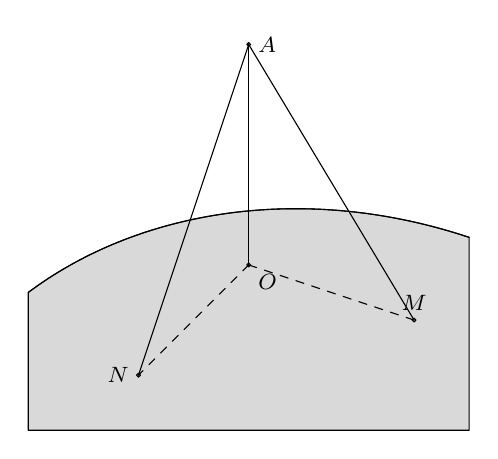
\begin{tikzpicture}[scale=0.7,font=\footnotesize,line join=round,line cap=round,>=stealth]
			\coordinate  (O) at (0,0);
			\coordinate (A)  at (0,4);
			\coordinate  (M) at (3,-1);
			\coordinate (N) at  (-2,-2);
			\draw[fill=gray!30,] (-4,-0.5).. controls (-2,1) and (1,1.5).. (4,0.5) -- (4,-3) -- (-4,-3)  -- cycle;
			\draw (-4,-0.5).. controls (-2,1) and (1,1.5)..  (4,0.5);
			 \draw (O) -- (A);
			\draw (A) --  (M);
			\draw  (A) -- (N);
			 \draw[dashed] (O) -- (M);
			\draw[dashed]  (O) -- (N);
			\draw (O) circle (1pt)  node[below right] {$O$};
			\draw (A) circle (1pt) node[right]  {$A$};
			\draw (M) circle (1pt)  node[above] {$M$};
			\draw (N) circle (1pt)  node[left] {$N$};
		\end{tikzpicture}
	} 
	\loigiai{ 
		Ta có $\overrightarrow{MA}  = (-4;6;5)$, $\overrightarrow{OM} = (4;-6;3)$, $\overrightarrow{ON} = (-4;-3;2) \Rightarrow \left[\overrightarrow{OM}, \overrightarrow{ON}\right] = (-3;-20;-36)$.\\
		Mặt phẳng sườn đồi $(OMN)$ có vectơ pháp tuyến $\overrightarrow{n} = \left[\overrightarrow{OM},  \overrightarrow{ON}\right] = (-3;-20;-36)$.\\
		Ta  có
		\begin{eqnarray*}
			\sin\left(MA,(OMN)\right) &=&\left|\cos\left(\overrightarrow{MA}, \overrightarrow{n}\right)\right|\\ 
			&=&\dfrac{\left|\overrightarrow{MA}\cdot \overrightarrow{n}\right|}{\left|\overrightarrow{MA}\right|\cdot \left|\overrightarrow{n}\right|}\\ 
			&=&\dfrac{\left|-4\cdot (-3)+6\cdot (-20)+5\cdot  (-36)\right|}{\sqrt{(-4)^2+6^2+5^2}\cdot \sqrt{(-3)^2+(-20)^2+(-36)^2}}= \dfrac{288}{\sqrt{131\,285}}.
		\end{eqnarray*}
		Suy ra  $\alpha \approx 53^\circ$.
	 }
\end{bt}


%%%%%%%%%%%%%%%% TỰ LUẬN %%%%%%%%%%%%%%%%

% nguồn: Phan2_Lop_12_Hinh_hoc_Chuong_5
\begin{bt}%[2H5H2-4]%[ma:90759c4c]
	Trong không gian $Oxyz$, xét vị trí tương  đối của các cặp đường thẳng sau:
	\begin{listEX}
		\item $d \colon \heva{&x=1+t\\&y=2t\\&z=3-t}(t\in\mathbb{R})$ và $d' \colon \heva{&x=2+2t'\\&y=3+4t'\\&z=5-2t'}(t'\in\mathbb{R})$. 
		\item  $d \colon \heva{&x=1+2t\\&y=-1+3t\\&z=5+t}(t\in\mathbb{R})$ và $d' \colon \dfrac{x-1}{3}=\dfrac{y+2}{2}=\dfrac{z+1}{2}$.
		\item $d  \colon \dfrac{x}{1}=\dfrac{y-1}{-1}=\dfrac{z}{2}$ và $d' \colon \dfrac{x-1}{5}=\dfrac{y-2}{1}=\dfrac{z+2}{-2}$.
	 \loigiai{
			\begin{listEX}
				\item Ta có các vectơ  chỉ phương của $d$ và $d'$ lần lượt là $\vec{a}=(1;2;-1)$ và $\vec{a}'=(2;4;-2)$.\\
				Vì $\vec{a}'=2\vec{a}$ nên $\vec{a}$ và $\vec{a}'$ cùng phương $\Rightarrow d$ và $d'$ song  song với nhau hoặc trùng nhau.\\
				Xét điểm $M(1;0;3)\in d$ và ta có $M\notin d'$ nên  $d \parallel d'$.
				\item Ta có $d$ và $d'$ lần lượt nhận $\vec{a}=(2;3;1)$ và $\vec{a}'=(3;2; 2)$ là các vectơ chỉ phương.\\ 
				Vì $\vec{a}$  và $\vec{a}'$ không cùng phương nên $d$ và $d'$ cắt nhau hoặc chéo nhau.
				Đường thẳng $d'$ qua $M(1;-2;-1)$; có VTCP $\vec{a}'=(3;2;2)$ nên có  phương trình là
				$d \colon \heva{&x=1+3t'\\&y=-2+2t'\\&z=-1+2t'}$.\\ 
				Xét hệ phương trình:  $\heva{&1+2t=1+3t'\\&-1+3t=-2+2t'\\&5+t=-1+2t'}\Leftrightarrow\heva{&t=\dfrac{-3}{5}\\&t'=\dfrac{-2}{5}\\&5+t=-1+2t'}\Rightarrow$ hệ vô nghiệm.\\
				Vậy hai đường thẳng $d$ và $d'$  chéo nhau.
				\item Ta có: $d$ đi qua $M(0; 1; 0)$ và có vectơ chỉ  phương $\vec{a}=(1;-1; 2)$. Đường thẳng $d'$ đi qua $M'(1; 2;-2)$ và có vectơ chỉ phương $\vec{a}'=(5; 1;-2)$.
				Nên phương trình tham số  của $d$ và $d'$ lần lượt là
				$$d \colon \heva{&x=t\\&y=1-t\\&z=2t}\text{ và }d' \colon \heva{&x=1+5t'\\&y=2+t'\\&z=-2-2t'}$$ 
				Xét hệ phương trình $\heva{&t=1+5t'\\&1-t=2+t'\\&2t=-2-2t'}\Leftrightarrow\heva{&t=\dfrac{-2}{3}\\&t'=\dfrac{-1}{3}}\Rightarrow$  hệ có nghiệm duy nhất.\\
				Vậy hai đường thẳng $d$  và $d'$ cắt nhau.
			\end{listEX}
		} 
	\end{listEX}
\end{bt}

% nguồn: Phan2_Lop_12_Hinh_hoc_Chuong_5
\begin{bt}%[2H5H2-4]%[ma:b2545ca7]
	Trong không gian với hệ toạ độ $Oxyz$, viết các  phương trình tham số và chính tắc của đường thẳng $\Delta$ đi qua $A(1;1;2)$ và song song với đường thẳng $d \colon \dfrac{x-3}{2}=\dfrac{y-1}{1}=\dfrac{z+5}{3}$.
	 \loigiai{
		Đường thẳng  $d$ có vectơ chỉ phương là $\overrightarrow{u}=(2;1;3)$. \\
		 Vì $\Delta \parallel d$ nên vectơ chỉ phương của $\Delta$ là $\overrightarrow{u}=(2;1;3)$. \\
		Đường thẳng $\Delta$ đi qua điểm $A(1;1;2)$ và có vectơ chỉ phương là $\overrightarrow{u}=(2;1;3)$. \\ 
		Phương trình tham số của $\Delta$ là 
		$\heva{&x=1+2t \\ &y=1+t \\ &z=2+3t} \quad  (t \in \mathbb{R})$. \\
		Phương trình chính tắc  của $\Delta$ là
		 $\dfrac{x-1}{2}=\dfrac{y-1}{1}=\dfrac{z-2}{3}$.
	 }
\end{bt}

% nguồn: Phan2_Lop_12_Hinh_hoc_Chuong_5
\begin{bt}%[2H5H2-4]%[ma:63a98635]
	Trong không gian với  hệ toạ độ $Oxyz$, cho hai đường thẳng
	\[ 
	\Delta_1\colon \heva{&x=1+2t \\ &y=3-t \\  &z=2+3t}
	\quad \text{  và} \quad
	\Delta_2  \colon \dfrac{x-8}{-1}=\dfrac{y+2}{1}=\dfrac{z-2}{2}.
	 \]
	\begin{itemize}
		 \item [a)] Chứng minh rằng $\Delta_1$ và $\Delta_2$ cắt nhau.
		\item [b)]  Viết phương trình mặt phẳng $(P)$ chứa $\Delta_1$ và $\Delta_2$.
	\end{itemize}
	 \loigiai{
		\begin{itemize}
			\item [a)] Đường thẳng $\Delta_1$ đi qua điểm $A(1;3;2)$ và có vectơ chỉ phương $\overrightarrow{u}_1=(2;-1;3)$. \\ 
			Đường thẳng $\Delta_2$ đi qua điểm $B(8;-2;2)$ và có vectơ  chỉ phương $\overrightarrow{u}_2=(-1;1;2)$. \\
			Ta có $\overrightarrow{AB}=(7;-5;0)$ và $\left[\overrightarrow{u}_1, \overrightarrow{u}_2\right]=(-5;-7;1) \ne \overrightarrow{0}  \quad (1)$. \\
			Mặt khác $\overrightarrow{AB} \cdot \left[\overrightarrow{u}_1,  \overrightarrow{u}_2\right]=-35+35=0 \quad (2)$. \\
			Từ (1) và (2) suy ra  $\Delta_1$ và $\Delta_2$ cắt nhau.
			\item [b)] Mặt phẳng $(P)$ chứa $\Delta_1$ và $\Delta_2$ nên có một vectơ pháp tuyến là $\overrightarrow{n}=\left[\overrightarrow{u}_1,  \overrightarrow{u}_2\right]=(-5;-7;1)$. \\
			Mặt  phẳng $(P)$ đi qua điểm $A(1;3;2)$ có vectơ pháp tuyến $\overrightarrow{n}=(-5;-7;1)$, có phương trình là
			 \[
			-5(x-1)-7(y-3)+(z-2)=0  \Leftrightarrow 5x+7y-z-24=0.
			\] 
		\end{itemize}
	 }
\end{bt}

% nguồn: Ok_TuanLuan_Toan11_Lan2
\begin{ex}%[2H5V2-4]%[ma:8723cef8]
	Cho hình chóp $S.ABCD$ có đáy $ABCD$ là hình vuông cạnh bằng $10$. Cạnh bên $SA$ vuông góc với mặt phẳng $(ABCD)$ và $SC = 10\sqrt{5}$. Gọi $M, N$ lần lượt là trung  điểm của $SA$ và $CD$. Tính khoảng cách $d$ giữa $BD$ và $MN$.
	\loigiai{ 
		Xét tam giác  vuông $SAC$ có
		 $$
		 SA = \sqrt{SC^2 - AC^2} = \sqrt{500 - 200} = 10\sqrt{3}.
		$$ 
		Chọn hệ trục  tọa độ như hình vẽ sao cho\\
		$ 
		A(0;0;0)$, $ B(10;0;0)$,  $ D(0;10;0)$, $ C(10;10;0)$, $ S\left(0;0;10\sqrt{3}\right)$, $
		 M(0;0;5\sqrt{3})$, $N(5;10;0).$
		\begin{center}
			\tdplotsetmaincoords{70}{110} 
			\begin{tikzpicture}[tdplot_main_coords,scale=1]
					\coordinate (A) at (0,0,0); 
					\coordinate (B) at (4,0,0); 
					\coordinate (C) at (4,4,0); 
					\coordinate  (D) at (0,4,0);
					\coordinate (S) at  (0,0,4);
					\draw[dashed] (A) --  (D);
					\draw[dashed] (A) -- (B); 
					\draw (B) -- (C)  -- (D);
					\draw[dashed] (S)  -- (A);
					\draw (S) -- (B); 
					\draw (S) -- (C); 
					\draw (S)  -- (D);
					\node at  (A) [left] {$A$};
					\node at  (B) [above left] {$B$};
					\node at (C) [below  right] {$C$};
					\node at  (D) [above right] {$D$};
					\node at (S)  [left] {$S$};
					\coordinate (M) at ($(S)!0.5!(A)$); 
					\coordinate  (N) at ($(C)!0.5!(D)$);
					\fill (M) circle (1pt) node[left]  {$M$};
					\fill  (N) circle (1pt) node[right] {$N$};
					\draw[dashed] (B) --  (D);
					\draw[dashed] (M) --  (N);
					\draw[->] (B) --  (5,0,0) node[right] {$x$};
					 \draw[->] (D) -- (0,5,0) node[above] {$y$};
					\draw[->] (S) -- (0,0,5) node[above] {$z$}; 
				\end{tikzpicture}
		\end{center}
		Ta  có
		\begin{itemize}
			\item $\vec{MN} = (5;10;-5\sqrt{3}) \Rightarrow \vec{u}_1 =  (1;2;-\sqrt{3})$.
			 \item $ \vec{BD} = (-10;10;0) \Rightarrow \vec{u}_2 = (-1;1;0)$.
		\end{itemize}
		Ta có 
		$$ 
		\left[\vec{u}_1,  \vec{u}_2\right] =
		\left(\sqrt{3};  \sqrt{3}; 3\right)
		\quad \text{và} \quad \vec{ND} = (-5;0;0). 
		$$ 
		 $$
		 \Rightarrow \mathrm{d}(MN, BD) = \dfrac{\left|\left[\vec{u}_1, \vec{u}_2\right] \cdot \vec{ND}\right|}{\left|\left[\vec{u}_1, \vec{u}_2\right]\right|} = \dfrac{\left|-\sqrt{3} \cdot 5\right|}{\sqrt{3^2 + 3 + 3}} = \dfrac{5\sqrt{3}}{\sqrt{9 + 3 + 3}} = \sqrt{5}.
		 $$
	} 
\end{ex}

% nguồn: Ok_TuanLuan_Toan11_Lan2
\begin{ex}%[2H5V2-4]%[ma:a906e65e]
	Cho hình lập phương $ABCD.A'B'C'D'$ có cạnh  bằng $a$. Gọi $K$ là trung điểm của $DD'$. Khoảng cách giữa hai đường thẳng $CK$ và $A'D'$ bằng bao nhiêu?
	 \loigiai{
		Chọn hệ trục tọa độ $Oxyz$ sao  cho
		 $
		D(0;0;0)$,  $A'(a;0;a)$, $ K\left(0;0;\dfrac{a}{2}\right)$, $ C(0;a;0)$.
		\begin{center}
			\tdplotsetmaincoords{70}{120} 
			\begin{tikzpicture}[tdplot_main_coords,scale=3.5]
					\pgfmathsetmacro{\a}{1} 
					\coordinate (D) at (0,0,0); 
					 \coordinate (A) at (\a,0,0);
					 \coordinate (C) at (0,\a,0);
					\coordinate (B) at  (\a,\a,0);
					\coordinate (D')  at (0,0,\a);
					\coordinate (A') at  (\a,0,\a);
					 \coordinate (C') at (0,\a,\a);
					 \coordinate (B') at (\a,\a,\a);
					\coordinate  (K) at (0,0,0.5*\a);
					\draw[dashed] (D)  -- (A);
					\draw[dashed]  (D) -- (C);
					\draw[dashed]  (D) -- (D');
					\draw  (A) -- (B);
					\draw (B) -- (C); 
					\draw (A)  -- (A');
					\draw (B) --  (B');
					\draw (C) -- (C'); 
					\draw (D')  -- (A');
					\draw (D')  -- (C');
					\draw (A')  -- (B');
					\draw (B')  -- (C');
					 \draw[dashed] (C) -- (K);
					 \draw[dashed] (A') -- (D);
					\draw[->] (A) --  (1.5*\a,0,0) node[below] {$x$};
					\draw[->] (C)  -- (0,1.5*\a,0) node[right] {$y$};
					\draw[->] (D') --  (0,0,1.5*\a) node[above] {$z$};
					\foreach  \point/\pos in {A/left,B/below right,C/above right,D/left,
						A'/left,B'/below  right,C'/right,D'/left,K/left}
					\fill (\point) circle  (0.5pt) node[\pos] {$\point$};
				\end{tikzpicture}
		\end{center}
		Ta  có
		 $$
		\vec{DA'} = (a;0;a),\quad  \vec{CK} = \left(0;-a;\dfrac{a}{2}\right),\quad \vec{DK} = \left(0;0;\dfrac{a}{2}\right).
		$$ 
		 Khi đó
		\begin{eqnarray*}
			 & &\left[\vec{DA'}, \vec{CK}\right]
			= \left(a^2; -\dfrac{a^2}{2}; -a^2\right)=a^2\left(-1;-\dfrac{1}{2};-1\right).\\ 
			& &\left[\vec{DA'}, \vec{CK}\right] \cdot \vec{DK} = a^2\cdot\left(1;  -\dfrac{1}{2}; -1\right) \cdot \left(0; 0; \dfrac{a}{2}\right) = -\dfrac{a^3}{2}.
		\end{eqnarray*}
		Do  đó
		 $$
		\mathrm{d}\left(A'D',  CK\right) = \dfrac{\left|\left[\vec{DA'}, \vec{CK}\right] \cdot \vec{DK}\right|}{\left|\left[\vec{DA'}, \vec{CK}\right]\right|} =
		\dfrac{\dfrac{a^3}{2}}{a^2\sqrt{1^2 + \left(\dfrac{1}{2}\right)^2 + 1^2}} = \dfrac{\dfrac{a}{2}}{\sqrt{1 + \dfrac{1}{4} +  1}} = \dfrac{a}{3}.
		$$ 
	} 
\end{ex}

% nguồn: Ok_TuanLuan_Toan11_Lan2
\begin{ex}%[2H5V2-4]%[ma:fa2c804c]
	Cho hình chóp $S.ABCD$ có đáy $ABCD$ là hình vuông cạnh $a$. Cạnh bên $SA$ vuông góc với đáy. Góc giữa $SC$ và mặt đáy bằng $45^\circ$. Gọi $E$ là trung điểm $BC$. Tính khoảng cách  giữa hai đường thẳng $DE$ và $SC$.
	\loigiai{ 
		Do tam giác $SCA$ vuông tại $A$, góc $\widehat{SCA} = 45^\circ$ nên 
		 $$
		SA = AC = a\sqrt{2}, \quad SC = 2a,\quad SB  = SD = a\sqrt{3}.
		$$ 
		Chọn hệ trục tọa độ $Oxyz$ sao cho $Ox$, $Oy$, $Oz$ lần lượt trùng  với các tia $AB$, $AD$, $AS$.\\
		Tọa độ các  điểm
		$ 
		D(0; a; 0)$, $E\left(a; \dfrac{a}{2}; 0\right)$, $C(a; a; 0)$, $ S\left(0; 0;  a\sqrt{2}\right).
		$ 
		\begin{center}
			\tdplotsetmaincoords{70}{110} 
			\begin{tikzpicture}[tdplot_main_coords,scale=1.4]
					\coordinate (A) at (0,0,0); 
					\coordinate (B) at (3,0,0); 
					 \coordinate (D) at (0,3,0);
					\coordinate (C)  at (3,3,0);
					\coordinate (S) at (0,0,3.24); 
					\coordinate (E) at ($(B)!0.5!(C)$); 
					\coordinate (M)  at ($(S)!0.5!(B)$);
					\draw[dashed]  (B) -- (A) -- (D);
					 \draw (B) -- (C) -- (D);
					 \draw[dashed] (S) -- (A);
					\draw (S) -- (B); 
					\draw  (S) -- (D);
					\draw (S) --  (C);
					\draw[dashed] (M) --  (D) -- (E);
					\draw (S) --  (C);
					\draw  (S) -- (M);
					\draw (B) -- (M)  -- (E);
					\node at (A) [below]  {$A$};
					\node at (B) [below right] {$B$}; 
					 \node at (C) [below right] {$C$};
					\node at (D) [below right] {$D$}; 
					 \node at (S) [left] {$S$};
					\node  at (E) [below right] {$E$};
					 \node at (M) [above right] {$M$};
					\draw[->] (B) -- (4.5,0,0) node[below] {$x$}; 
					\draw[->]  (D) -- (0,4.5,0) node[above] {$y$};
					\draw[->] (S)  -- (0,0,4) node[above] {$z$};
					\fill  (A) circle (1pt);
					 \fill (B) circle (1pt);
					\fill (C) circle  (1pt);
					 \fill (D) circle (1pt);
					\fill (S)  circle (1pt);
					 \fill (E) circle (1pt);
					\fill  (M) circle (1pt);
				\end{tikzpicture}
		\end{center}
		Ta  có
		$ 
		\vec{DE} = \left(a, -\dfrac{a}{2}, 0\right)$, $ \vec{SC} = \left(-a, -a, a\sqrt{2}\right)$, $ \vec{DC} =  (a, 0, 0)$.
		\begin{eqnarray*}
			& & \left[\vec{DE}, \vec{SC}\right] = 
			\left(-\dfrac{a^2\sqrt{2}}{2}; -a^2\sqrt{2};  -\dfrac{3a^2}{2} \right).\\
			& & \left[\vec{DE}, \vec{SC}\right] \cdot \vec{DC} = \left(-\dfrac{a^2\sqrt{2}}{2}; -a^2\sqrt{2}; -\dfrac{3a^2}{2} \right)  \cdot (a; 0; 0) = -\dfrac{a^3\sqrt{2}}{2}.\\
			&\Rightarrow&\mathrm{d}(DE, SC) = \dfrac{\left|\left[\vec{DE}, \vec{SC}\right] \cdot \vec{DC}\right|}{\left|\left[\vec{DE}, \vec{SC}\right]\right|} = \dfrac{\dfrac{a^3\sqrt{2}}{2}}{\sqrt{\left(\dfrac{a^2\sqrt{2}}{2}\right)^2 + \left(a^2\sqrt{2}\right)^2 + \left(\dfrac{3a^2}{2}\right)^2}}  = \dfrac{a\sqrt{38}}{19}.
		\end{eqnarray*}
	} 
\end{ex}

% nguồn: Phan2_Lop_12_Hinh_hoc_Chuong_5
\begin{bt}%[2H5V2-4]%[ma:85b1b6f3]
	Cho hình chóp $S.ABCD$ có đáy $ABCD$ là hình vuông cạnh bằng $10$. Cạnh bên $SA$ vuông góc với mặt phẳng $(ABCD)$ và $SC = 10\sqrt{5}$. Gọi $M, N$ lần lượt là trung điểm của $SA$ và $CD$. Tính khoảng cách $d$ giữa  $BD$ và $MN$.
	 \loigiai{
		Xét tam giác vuông $SAC$ có 
		$$ 
		SA = \sqrt{SC^2 - AC^2} = \sqrt{500  - 200} = 10\sqrt{3}.
		$$ 
		Chọn hệ  trục tọa độ như hình vẽ sao cho\\
		$ 
		A(0;0;0)$, $  B(10;0;0)$, $ D(0;10;0)$, $ C(10;10;0)$, $ S\left(0;0;10\sqrt{3}\right)$, $
		M(0;0;5\sqrt{3})$, $N(5;10;0).$ 
		\begin{center}
			\tdplotsetmaincoords{70}{110} 
			\begin{tikzpicture}[tdplot_main_coords,scale=1]
					\coordinate (A) at (0,0,0); 
					\coordinate  (B) at (4,0,0);
					\coordinate (C)  at (4,4,0);
					\coordinate (D) at (0,4,0); 
					\coordinate  (S) at (0,0,4);
					\draw[dashed] (A) --  (D);
					\draw[dashed] (A)  -- (B);
					\draw  (B) -- (C) -- (D);
					\draw[dashed] (S) --  (A);
					\draw  (S) -- (B);
					 \draw (S) -- (C);
					\draw (S) --  (D);
					\node  at (A) [left] {$A$};
					\node at (B) [above  left] {$B$};
					\node at (C) [below right]  {$C$};
					\node at (D) [above right]  {$D$};
					\node at (S) [left]  {$S$};
					\coordinate (M)  at ($(S)!0.5!(A)$);
					\coordinate (N) at ($(C)!0.5!(D)$); 
					\fill  (M) circle (1pt) node[left] {$M$};
					\fill (N) circle (1pt) node[right] {$N$}; 
					\draw[dashed] (B) -- (D); 
					\draw[dashed] (M) --  (N);
					\draw[->] (B) -- (5,0,0)  node[right] {$x$};
					\draw[->] (D) -- (0,5,0) node[above] {$y$}; 
					\draw[->]  (S) -- (0,0,5) node[above] {$z$};
				\end{tikzpicture}
		\end{center}
		Ta có 
		\begin{itemize}
			\item $\vec{MN}  = (5;10;-5\sqrt{3}) \Rightarrow \vec{u}_1 = (1;2;-\sqrt{3})$.
			\item $ \vec{BD} =  (-10;10;0) \Rightarrow \vec{u}_2 = (-1;1;0)$.
		\end{itemize}
		 Ta có
		 $$
		 \left[\vec{u}_1, \vec{u}_2\right] =
		\left(\sqrt{3};  \sqrt{3}; 3\right)
		\quad  \text{ và} \quad \vec{ND} = (-5;0;0).
		$$ 
		$$ 
		\Rightarrow  \mathrm{d}(MN, BD) = \dfrac{\left|\left[\vec{u}_1, \vec{u}_2\right] \cdot \vec{ND}\right|}{\left|\left[\vec{u}_1, \vec{u}_2\right]\right|} = \dfrac{\left|-\sqrt{3} \cdot 5\right|}{\sqrt{3^2 + 3 + 3}} = \dfrac{5\sqrt{3}}{\sqrt{9 + 3 + 3}} = \sqrt{5}.
		$$ 
	 }
\end{bt}

% nguồn: Phan2_Lop_12_Hinh_hoc_Chuong_5
\begin{bt}%[2H5V2-4]%[ma:116b23aa]
	Cho hình chóp $S.ABCD$ có đáy $ABCD$ là hình vuông cạnh $a$. Cạnh bên $SA$ vuông góc với đáy. Góc giữa $SC$ và mặt đáy bằng  $45^\circ$. Gọi $E$ là trung điểm $BC$. Tính khoảng cách giữa hai đường thẳng $DE$ và $SC$.
	 \loigiai{
		Do tam giác $SCA$ vuông tại $A$,  góc $\widehat{SCA} = 45^\circ$ nên
		$$ 
		SA = AC = a\sqrt{2}, \quad SC = 2a,\quad SB = SD = a\sqrt{3}. 
		 $$
		Chọn hệ trục tọa độ $Oxyz$ sao cho $Ox$, $Oy$, $Oz$  lần lượt trùng với các tia $AB$, $AD$, $AS$.\\
		Tọa  độ các điểm
		 $
		 D(0; a; 0)$, $E\left(a; \dfrac{a}{2}; 0\right)$, $C(a; a; 0)$, $ S\left(0; 0; a\sqrt{2}\right).
		$ 
		\begin{center}
			\tdplotsetmaincoords{70}{110} 
			\begin{tikzpicture}[tdplot_main_coords,scale=1.4]
					 \coordinate (A) at (0,0,0);
					\coordinate (B) at (3,0,0); 
					\coordinate  (D) at (0,3,0);
					\coordinate (C) at (3,3,0); 
					 \coordinate (S) at (0,0,3.24);
					 \coordinate (E) at ($(B)!0.5!(C)$);
					\coordinate (M)  at ($(S)!0.5!(B)$);
					\draw[dashed] (B) --  (A) -- (D);
					\draw (B) -- (C) --  (D);
					 \draw[dashed] (S) -- (A);
					\draw (S) --  (B);
					\draw (S) -- (D); 
					 \draw (S) -- (C);
					 \draw[dashed] (M) -- (D) -- (E);
					 \draw (S) -- (C);
					\draw (S)  -- (M);
					\draw (B) -- (M) --  (E);
					\node at  (A) [below] {$A$};
					 \node at (B) [below right] {$B$};
					\node at (C) [below right] {$C$}; 
					\node at (D)  [below right] {$D$};
					\node at (S)  [left] {$S$};
					 \node at (E) [below right] {$E$};
					 \node at (M) [above right] {$M$};
					\draw[->] (B) --  (4.5,0,0) node[below] {$x$};
					\draw[->] (D)  -- (0,4.5,0) node[above] {$y$};
					 \draw[->] (S) -- (0,0,4) node[above] {$z$};
					\fill (A) circle (1pt); 
					\fill (B) circle (1pt); 
					 \fill (C) circle (1pt);
					\fill (D) circle  (1pt);
					\fill (S) circle  (1pt);
					\fill (E) circle (1pt); 
					\fill (M) circle  (1pt);
				\end{tikzpicture}
		\end{center}
		 Ta có
		 $
		 \vec{DE} = \left(a, -\dfrac{a}{2}, 0\right)$, $ \vec{SC} = \left(-a, -a, a\sqrt{2}\right)$, $ \vec{DC} = (a, 0, 0)$.
		\begin{eqnarray*}
			& & \left[\vec{DE},  \vec{SC}\right] =
			\left(-\dfrac{a^2\sqrt{2}}{2}; -a^2\sqrt{2}; -\dfrac{3a^2}{2}  \right).\\
			& & \left[\vec{DE}, \vec{SC}\right] \cdot \vec{DC} = \left(-\dfrac{a^2\sqrt{2}}{2}; -a^2\sqrt{2}; -\dfrac{3a^2}{2} \right)  \cdot (a; 0; 0) = -\dfrac{a^3\sqrt{2}}{2}.\\
			&\Rightarrow&\mathrm{d}(DE, SC) = \dfrac{\left|\left[\vec{DE},  \vec{SC}\right] \cdot \vec{DC}\right|}{\left|\left[\vec{DE}, \vec{SC}\right]\right|} = \dfrac{\dfrac{a^3\sqrt{2}}{2}}{\sqrt{\left(\dfrac{a^2\sqrt{2}}{2}\right)^2 + \left(a^2\sqrt{2}\right)^2 + \left(\dfrac{3a^2}{2}\right)^2}} = \dfrac{a\sqrt{38}}{19}.
		\end{eqnarray*}
	 }
\end{bt}
